%% ----------------------------------------------------------------
%% Thesis.tex -- MAIN FILE (the one that you compile with LaTeX)
%% ---------------------------------------------------------------- 

% Set up the document
\documentclass[a4paper, 8pt, oneside]{Thesis}  % Use the "Thesis" style, based on the ECS Thesis style by Steve Gunn
\graphicspath{Figures/}  % Location of the graphics files (set up for graphics to be in PDF format)
\usepackage[english]{babel}
\usepackage[utf8x]{inputenc}
\usepackage{amsmath}
\usepackage{graphicx}
\usepackage{hyperref}
\usepackage[]{algorithmicx}
%\usepackage{lipsum}
%\usepackage[]{classicthesis}
\usepackage[table]{xcolor}
\usepackage{tabularx}
\usepackage[nottoc]{tocbibind}
% Include any extra LaTeX packages required
\usepackage[square, numbers, comma, sort&compress]{natbib}  % Use the "Natbib" style for the references in the Bibliography
\usepackage{verbatim}  % Needed for the "comment" environment to make LaTeX comments
\usepackage{vector}  % Allows "\bvec{}" and "\buvec{}" for "blackboard" style bold vectors in maths
\hypersetup{urlcolor=blue, colorlinks=true}  % Colours hyperlinks in blue, but this can be distracting if there are many links.
\usepackage{color}
\lstset{ %
language=C++,                % choose the language of the code
basicstyle=\footnotesize,       % the size of the fonts that are used for the code
numbers=left,                   % where to put the line-numbers
numberstyle=\footnotesize,      % the size of the fonts that are used for the line-numbers
stepnumber=1,                   % the step between two line-numbers. If it is 1 each line will be numbered
numbersep=5pt,                  % how far the line-numbers are from the code
backgroundcolor=\color{white},  % choose the background color. You must add \usepackage{color}
showspaces=false,               % show spaces adding particular underscores
showstringspaces=false,         % underline spaces within strings
showtabs=false,                 % show tabs within strings adding particular underscores
frame=single,           % adds a frame around the code
tabsize=2,          % sets default tabsize to 2 spaces
captionpos=b,           % sets the caption-position to bottom
breaklines=true,        % sets automatic line breaking
breakatwhitespace=false,    % sets if automatic breaks should only happen at whitespace
escapeinside={\%*}{*)}          % if you want to add a comment within your code
}
%% ----------------------------------------------------------------
\begin{document}
\begin{titlepage}

\newcommand{\HRule}{\rule{\linewidth}{0.5mm}} % Defines a new command for the horizontal lines, change thickness here

\center % Center everything on the page
 
%----------------------------------------------------------------------------------------
%	HEADING SECTIONS
%----------------------------------------------------------------------------------------

\textsc{\LARGE Università della Svizzera italiana}\\[1.5cm] % Name of your university/college
\textsc{\large GPU Implementation of the  Lean Algebraic Multi-grid (LAMG) Solver for Large-scale Graph Problems}\\[0.5cm] % Major heading such as course name
\textsc{ }\\[0.5cm] % Minor heading such as course title

%----------------------------------------------------------------------------------------
%	TITLE SECTION
%----------------------------------------------------------------------------------------

\HRule \\[0.4cm]
{ \huge \bfseries Bachelor Project}\\[0.4cm] % Title of your document
\HRule \\[1.5cm]
 
%----------------------------------------------------------------------------------------
%	AUTHOR SECTION
%----------------------------------------------------------------------------------------

\begin{minipage}{0.4\textwidth}
\begin{flushleft} \large
\emph{Author:}\\
Satish \textsc{Kumar} % Your name
\end{flushleft}
\end{minipage}
~
\begin{minipage}{0.4\textwidth}
\begin{flushright} \large
\emph{Supervisor:} \\
Prof  \textsc{Rolf Krause}\\ % Supervisor's Name
\textsc{Riva Simone}
\end{flushright}
\end{minipage}\\[2cm]

% If you don't want a supervisor, uncomment the two lines below and remove the section above
%\Large \emph{Author:}\\
%John \textsc{Smith}\\[3cm] % Your name

%----------------------------------------------------------------------------------------
%	DATE SECTION
%----------------------------------------------------------------------------------------

{\large \today}\\[2cm] % Date, change the \today to a set date if you want to be precise

%----------------------------------------------------------------------------------------
%	LOGO SECTION
%----------------------------------------------------------------------------------------

\includegraphics[width=30mm]{../logo.png}\\[0.5cm] % Include a department/university logo - this will require the graphicx package
 
%----------------------------------------------------------------------------------------

\vfill % Fill the rest of the page with whitespace

\end{titlepage}
% Declaration Page required for the Thesis, your institution may give you a different text to place here


\addtocontents{toc}{\vspace{1em}}  % Add a gap in the Contents, for aesthetics
%% ----------------------------------------------------------------


\pagestyle{fancy}  %The page style headers have been "empty" all this time, now use the "fancy" headers as defined before to bring them back


%% ----------------------------------------------------------------
\lhead{\emph{Contents}}  % Set the left side page header to "Contents"
\tableofcontents  % Write out the Table of Contents
\clearpage

%% ----------------------------------------------------------------

\setstretch{1.5}  % Set the line spacing to 1.5, this makes the following tables easier to read
\clearpage  % Start a new page
\lhead{\emph{}}  % Set the left side page header to "Abbreviations"
\listofsymbols{ll}  % Include a list of Abbreviations (a table of two columns)
{
% \textbf{Acronym} & \textbf{W}hat (it) \textbf{S}tands \textbf{F}or \\
Graphic Processing Unit (GPU) has become one of the most important \\components in modern computer systems. GPUs have evolved from  a\\ single-purpose graphic rendering hardware to a powerful processor that\\ is capable of handling many different kinds of computing task.\\

In this report we have created linear algebra API using OCCA and C++.\\ We demonstrated that the individual linear algebra components \\can be faster when using the OCCA as compared to the CPU.\\
We have worked in OCCA because OCCA is a open-source library. \\It provide a kernel language, a minor extension to C. It is easy to understand.\\ OCCA supports device kernel expansion for the OpenCL, OpenMP and CUDA.\\ 

We implemented the matrix multiplication. Multiplication between matrix\\ and vector, Sparse matrix in CSR format, sparse matrix in CSR format with\\ vector multiplication, matrix - matrix addition, matrix - matrix subtraction,\\ dot product between vectors, with reduction and Multi-grid method for dense\\ matrix and sparse matrix. Thus we have analyzed and compared the performance\\ between OCCA and CPU.
}

%% ----------------------------------------------------------------
\mainmatter	  % Begin normal, numeric (1,2,3...) page numbering
\pagestyle{fancy}  % Return the page headers back to the "fancy" style

% Include the chapters of the thesis, as separate files
% Just uncomment the lines as you write the chapters

\chapter{Introduction}
In this chapter, We will explain the multi-grid definition and OCCA components. We are using CSR format for sparse matrix. We will explain also, What is CSR format ? and how can we save memory with using CSR format ?


\section{Multi-grid Method}
\subsection{Model Problem}
Multigrid methods were originally applied to simple boundary value problems that arise in many physical applications. For simplicity and for historical reasons, these problems provide a natural introduction to multi-grid methods.\\

\subsubsection{One-dimensional boundary value problem:}
\begin{equation}
	-u''(x) + \alpha u(x) = f(x)  \quad 0<c<1, \alpha > 0 
\end{equation}
\begin{equation}
	u(0) = u(1) = 0
\end{equation}

While this problem can be handled analytically, our present aim is to consider numerical methods. Many such approaches are possible, the simplest of which is a finite difference method. The domain of the problem ${x : 0\leq x\leq 1}$ is partitioned into n subintervals by introducing the grid points $X_j = j_h$, where h = 1/n is the constant width of the subintervals. which we denote h.
	At each of the n-1 interior grid points, the original differential equation (1.1) is replaced by a second-order finite difference approximation. In making this replacement, we also introduce as an approximation to the exact solution $U(X_j)$. This approximate solution may now be represented by a vector $v = (v_i,..., v_{n-i})^T$, whose components satisfy the n —l linear equations\\
	Defining $f=(f(x_1),...,f(x_{n_1}))^T =(f_1,...,f_{n-i})^T$, the vector of right-side values, we may also represent this system of linear equations in matrix form as\\
	$1/h^2
	\begin{bmatrix}
		2+\alpha h^2 & -1 & & & &\\
		-1 & 2+\alpha h^2 & -1 & & &\\
		&. & . & . & & \\
		& &. & . & . &  -1 \\
		 & & -1 & & -1 &2+\alpha h^2\\
	\end{bmatrix}
	\begin{bmatrix}
		v_1\\
		.\\
		.\\
		.\\
		v_{n-1}
	\end{bmatrix} = 
	\begin{bmatrix}
		f_1\\
		.\\
		.\\
		.\\
		f_{n-1}
	\end{bmatrix}$\\
	or even more compactly as Av = f. The matrix A is (n —1) x (n —1), tridiagonal, symmetric and positive definite.\\
	\subsubsection{Solution Methods} 
To solve the systems of linear equations there are several methods of solution:\\
• Direct\\
– Gaussian elimination \\
– Factorisation\\
• Iterative\\
– Jacobi\\
– Gauss-Seidel\\
– Conjugate Gradient, etc.\\
When it comes to choosing between direct or iterative solution methods, there are several factors to consider.\\
The first consideration is the application and the computer that is used. Since direct methods are expensive in terms of memory and time intensive for CPUs, they are preferable for small to medium-sized 2D and 3D applications. Conversely, iterative methods have a lower memory consumption and for large 3D applications, they outperform direct methods. Further, it is important to note that iterative methods are more difficult to tune and more challenging to get working for matrices arising from multi-physics problems. 
\subsubsection{A two-dimensional boundary value problem}
$-u''(xx) - u(yy) + \alpha u(x) = f(x,y)  \quad 0<x<1, \quad 0<y<1,\\
u = 0 , x = 0, x = 1, y = 0, y = 1 \quad  \alpha > 0$ \\ 
We obtain a block-tridiagonal system Av=f\\
$
	\begin{bmatrix}
		A_1 & -I_y & & & &\\
		-I_y & A_2 & -I_y & & &\\
		&. & . & . & & \\
		& &. & . & . &   \\
		 & &  & & -I_y &A_{N-1}\\
	\end{bmatrix}
	\begin{bmatrix}
		v_1\\
		.\\
		.\\
		.\\
		v_{N-1}
	\end{bmatrix} = 
	\begin{bmatrix}
		f_1\\
		.\\
		.\\
		.\\
		f_{N-1}
	\end{bmatrix}$\\
	where $I_y$ is a diagonal matrix with $1/h^2_y$ on the diagonal\\
	
	The main idea of multi-grid is to accelerate the convergence of a basic iterative method (known as relaxation, which generally reduces short-wavelength error) by a global correction of the fine grid solution approximation from time to time accomplished by solving a coarse problem. The coarse problem, while cheaper to solve is similar to the fine grid problem in that it also has short and long-wave length errors. It can also be solved by a combination of relaxation and appeal to still coarser grids. This recursive process is repeated until a grid is reached where the cost of direct solution there is negligible compared to the cost of one relaxation sweep on the fine grid. This multi-grid cycle typically reduces all error components by a fixed amount bounded well below one independent of the fine grid mesh size. The typical application for multi-grid is in the numerical solution of elliptic partial differential equations in two or more dimensions.\\
	There are many variations of multi-grid algorithms, but the common features are that a hierarchy of discretisations (grids) is considered. The important steps are:\\

Smoothing – reducing high frequency errors, for example using a few iterations of the Gauss–Seidel method.\\
Restriction – downsampling the residual error to a coarser grid.\\
Interpolation or prolongation – interpolating a correction computed on a coarser grid into a finer grid.\\
\subsubsection{Computation Costs}
Let 1 Work Unit(WU) be the cost of one relaxation sweep on the fine-grid.\\
• Ignore the cost of restriction and interpolation (typically about 20 percentage of the total cost).\\
• Consider a V-cycle with 1 pre-Coarse-Grid correction relaxation sweep and 1 post-Coarse- Grid correction relaxation sweep.\\
• Cost of V-cycle(in WU):\\
$2(1+2^{-d}+2^{-2d}+2^{-3d}+...+2^{-Md} < \dfrac{2}{1-2^{-d}}$\\
Cost is about 4,8/3,16/7 WU per V-cycle in 1,2 and 3 dimensions.\\
• Multi grid has been proven on a wide variety of problems, especially elliptic PDEs, but has also found application among parabolic $\&$ hyperbolic PDEs, integral equations, evolution problems, geodesic problems etc.\\
• With the right setup, multi grid is frequently an optimal (i.e., O(N)) solver.\\
• Multi grid is of great interest because it is one of the very few scalable algorithms, and can be parallelised readily and efficiently!\\


%\subsection{A Subsection}

\section{OCCA: Unified Approach To Multithreading Languages}
%\href{https://scholarship.rice.edu/bitstream/handle/1911/102233/TR15-04.pdf?sequence=1&isAllowed=y}{OCCA}
\subsection{History}
\href{https://scholarship.rice.edu/bitstream/handle/1911/102233/TR15-04.pdf?sequence=1&isAllowed=y}{OCCA} (like oca-rina) started off a project in  Tim Warburton's group. The group mainly worked high-order numerical methods, specifically on the algorithms to make them performant. During that time, they mainly focused on GPU programming using OpenCL and CUDA.

They had wrappers for OpenCL and CUDA to test implementations, which we almost always had 2 almost identical codes to run on NVIDIA and AMD GPUs. From \ref{txt:occa} 
\subsection{Overview}
The different projects mentioned have focused on creating some mapping between two or more programming languages for these assertors or switching between multiple platform for computation purpose. OCCA, a library including an API that abstracts back-ends and kernel languages from OpenMP, OpenCL and CUDA. From \ref{txt:occa} 
\begin{figure}
\centering
\includegraphics[width= 12cm]{../occa2}
\caption{ Current relationship between supported frontends, the OCCA languages, and supported backends}
\end{figure}\\
\subsection {Device}
Graphics cards were developed due to the increasing demand for improved graphics in video games. The similarities between CUDA and OpenCL become evident in their programming model but their popularity in use differ. NVIDIA releases their own compiler wrapper, nvcc to allow CUDA kernels to be embedded in the application code. While OpenCL separates host code (application code) with the device code (kernels), which steepens the learning curve.\\
\subsection {Setup device}
An implementation of this concept was developed, producing the OCCA intermediate representation (IR) which generalises current parallel architectures to unify the different languages and standards for heterogeneous computing, including serial code, Pthreads, OpenMP, CUDA, OpenCL \\



In OCCA we can define the \textbf{target device runtime}, with the following simples lines of codes. From \ref{txt:occa}  \\
\centerline{"mode: 'Serial'"}\\
We can used the device manually also\\
CUDA  \centerline{"mode: 'CUDA', deviceID: 0"}\\
OpenCL  \centerline{"mode: 'OpenCL', deviceID: 0, platformID: 0"}\\
THREADS  \centerline{"mode: 'Threads', threads: 4, pinnedCores: [0, 1, 2, 3]"}\\
OPENMP  \centerline{"mode: 'OpenMP', threads: 4"}  \\

\subsection{Memory management}
We can not allocate runtime memory in the device. Hence in the host, data is usually initialised either copied to the device, modified in the device by running a kernel.\\

In OCCA we can allocate memory, with the following simples lines of codes. \\
\begin{lstlisting}[language=C, caption=allocating memory to the device]
	// Copy a and b to the device
	occa::memory o_a  = device.malloc(entries * sizeof(float), a);
	occa::memory o_b  = device.malloc(entries * sizeof(float), b);
	// Don't initialise o_ab
	occa::memory o_ab = device.malloc(entries * sizeof(float))
\end{lstlisting}
In code Listing 1.1 line 2 and 3, We are allocating memory of size entries with type float and copy a and b to device. But in line 5, We are just allocate memory. Because we allocate this memory for our result and we are not copying anything to it.
\subsection{kernel}
Okl (Programming language use by OCCA) now has the feature to automatically assign working dimensions to the off-load model through the outer and inner loops. A kernel launch in OpenCL and CUDA are always separate from the kernel source, but maintain a connection through the working dimensions used in a kernel execution.\\
Kernel are build at runtime so we require 2 things\\
1. file name with the kernel source code \\
2. Name of the kernel in source code\\
\begin{lstlisting}[language=C, caption=call to kernel function]
	occa::kernel addVectors = device.buildKernel("addVectors.okl",
                                             "addVectors")
    // we call to kernel function
    addVectors(n, o_a, o_b, o_ab);
\end{lstlisting}
Above Listing 1.2, We are using function buildKernel for building kernel at runtime. In listing 1.2, addVectors.okl is a file name with extension okl and addVectors is the kernel function name. And next-step we call to kernel with its variables.\\
\textbf{Parallelism}\\
\label{txt:innerOuterloop}
OpenCL and CUDA are always separate from the kernel source, but maintain a connection through the working dimension used in a kernel execution. OCCA extends the C for-loops by adding a fourth statement (@outer/ @inner). Aside from showing the explicit loops, OCCA now has the feature to automatically assign working dimensions to the offload model through the outer and inner loops.
\begin{lstlisting}[language=C, caption=outer loop example]
	for (int i = 0; i < 3; ++i; @outer) {
  		work(i);
}
//should be expected to work regardless of the iteration ordering, such as:
work(0);
work(1);
work(2);
// and also 
work(2);
work(0);
work(1);
\end{lstlisting}
Since the execution order can be non-deterministic and in parallel, there shouldn't be any loop dependencies.\\
Distributing work between outer and inner loops is heavily dependent on the device architecture. Try aiming for a power of 2 size for inner-loop sizes to make use of vectorization. From \ref{txt:mainOCCA}
%\section{Compressed Row Storage (CRS)}
%A sparse matrix or sparse array is a matrix in which most of the elements are zero. The number  of zero-valued elements divided by total number of elements is called sparsity of the matrix. When storing and computing sparse matrix on device it is necessary to use the efficient algorithm and data structure. Because we can store sparse matrix in significantly in less storage.
%\subsection{Introduction}
%The Compressed Row and Column Storage formats are the most general. They make absolutely no assumptions about the sparsity structure of the matrix and they don't store any unnecessary elements. On the other hand, they are not very efficient, needing an indirect addressing step for every single scalar operation in a matrix-vector product or preconditioned solve. From \ref{txt:CSR}\\
%For CRS, we create 3 vectors and size of the vectors are length of non-zero elements of matrix. They are 
%\begin{itemize}
%	\item Non-zero elements of the matrix
%	\item column number for non-zero elements of the matrix
%	\item row number for non-zero elements of the matrix
%\end{itemize}
%\begin{center}
%	\includegraphics[width=12cm]{../sparse.png} 
%	\captionof{figure}{convert sparse matrix to CSR format}
%	\label{img:csrfo}
%\end{center}
%
%
%The \texttt{val}  (\ref{img:csrfo}) represents the non-zero values of the matrix, read first by row left to right, then by column top to bottom. The \texttt{colind} represents the column index corresponding to the values. The \texttt{rowptr} represents the indexes belonging to a row, it contains an index per row corresponding to an index in the two other vectors. It is clear that all indexes from this starting index and to the starting index of the next row will belong to the given row. The last index is the number of rows plus one, so the algorithm doesn’t have to check if we’re at the last row.
%

 % Introduction

\chapter{Dense Matrix}

In this chpater, We will discuss implementation about dense matrix. Dense matrix is a matrix, Which have mostly element are non zero. We will implement matrix- vector, matrix multiplication and matrix addition and subtraction in CPU and OCCA.

\section{Dense matrix - vector multiplication}
\subsection{Introduction}
Matrix vector multiplication computes the product of matrix and vector. We can perform multiplications between a matrix and vector when number of columns of matrix equal number of rows of vector. In mathematical term m*n dimensional matrix can be multiplied only n dimensional vector.The theoretical operation is shown below, matrix-vector multiplication output is m*1 dimensional vector.\\
Input data: dense matrix A
 of size m-by-n (with entries $a_{ij}$
), its vector cofactor x
 of dimension n (with components $x_i$
).

Output data: vector y
 of dimension m (with components $y_i$
).

Formulas of the method:
\begin{equation}
	y_i = \sum _{j=1}^{n} a_{ij}x_j \quad   i \in [1...m]
\end{equation}

%There also exists a block version of the method. However, this description treats only the pointwise version.
The basic idea with visualisation as below:
\begin{center}
	
\end{center}
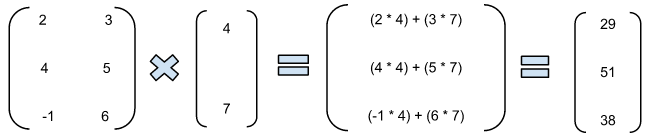
\includegraphics[width=12cm, height=2cm]{Chapters/matrix-vector-multiplication.png}
\captionof{figure}{matrix vector multiplication}
%\centerline{ 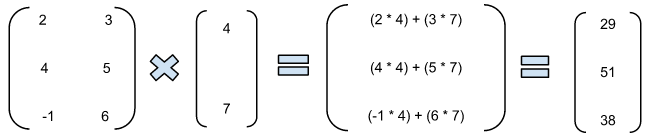
\includegraphics[width=12cm, height=2cm]{Chapters/matrix-vector-multiplication.png}}
\subsection{C++ implementation}
The C++ implementation is the most basic implementation. The idea is below\\

\begin{lstlisting}[language=C, caption=matrix vector multiplication in CPU/C++]
	we have m*n dimensional matrix
	for i < m;i++
		for j < n;j++
			result_vector[i] += matrix[i*n+j]*vector[j]
\end{lstlisting}

Listing 2.1 each iteration of the for loops, the code computes the product of two elements of matrix and vector and add the result. So the time complexity of the entire multiplication is $O(n^2)$, if we have matrix size n-by-n.




\subsection{OCCA implementation}
The OCCA utilises the data parallelism in matrix - vector multiplication.\\
\begin{lstlisting}[language=C, caption=matrix vector multiplication in OCCA]
	we have m*n dimensional matrix
	for i < m; i++;@tile(16, @outer, @inner)) // Work-group implicit loops
		for j < n;j++
			result_vector[i] += matrix[i*n+j]*vector[j]
\end{lstlisting}
In Listing 2.2, An additional tile tag was introduced to facilitate kernel development due to many kernels only requiring the use of simple bounds and iteration strides. The tile tag, tiling for-loops as one and two dimensional sets of inner/outer loops. The tile(16) assign the working dimension. In this example it assign the working dimension is 16. 
\subsection{OCCA vs CPU}

\begin{center}
	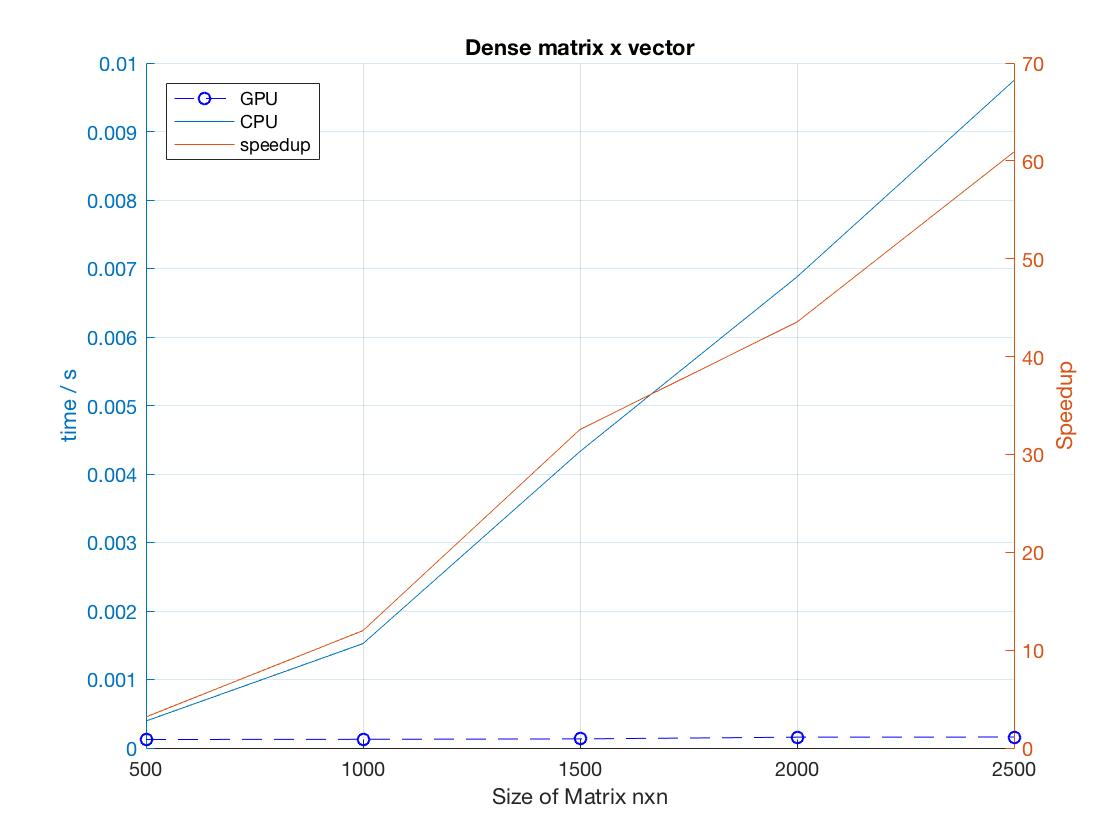
\includegraphics[width = 12cm]{chapters/dense_matrix_vector.jpg}
	\captionof{figure}{compare OCCA vs CPU performance}
	\label{img:1}
\end{center}

As we can see in figure \ref{img:1} OCCA always faster than CPU. If matrix and vector size is bigger than OCCA perform better than CPU.





\section{Dense matrix-matrix  multiplication}
\subsection{Introduction}
Matrix multiplication computes the product of two matrices. The theoretical operation show below, where matrix A and matrix B are the input matrices and produce the output matrix.\\
\begin{center}
	\includegraphics[width = 10cm]{../Matrix_multiplication}
	\captionof{figure}{matrix multiplication visualisation }
\end{center}

Let C is output matrix then mathematical formulation of the equation is
\begin{equation}
	C_{ij}=a_{i1}b_{1j}+\cdots +a_{im}b_{mj}=\sum _{k=1}^{m}a_{ik}b_{kj}
\end{equation}
for i = 1, ..., n and j = 1, ..., p.\\
That is, the entry $C_{ij}$ of the product is obtained by multiplying term-by-term the entries of the $i^{th}$ row of A and the $j^{th}$ column of B and summing these m products. In other words, $C_{ij}$ is the dot product of the $i^{th}$ row of A and the $j^{th}$ column of B.

\subsection{C++ implementation}
The C++ implementation is the most basic implementation. The pseudo code is below
\begin{lstlisting}[language=C, caption=matrix multiplication in CPU/C++]
	we have  m*n and n*m dimensional matrices
	for i < m; i++
		for j <m; j++
			for k < n;k++
				result[i][j] += A[i][k]*B[k][j]
\end{lstlisting}
In Listinig 2.3 , each iteration of the for loops, the code computes the product of two elements from matrix A and matrix B and add the product to the result from previous iteration of the loops. For example m by m square matrix to compute the element in result matrix, the CPU performs m multiply operations and n-1 sum operations. So the time complexity of entire multiplication there are $O(n^3)$ multiply operations and $O(n^2)$ sum operations.

\subsection{OCCA implementation}
The OCCA utilises the parallelism in matrix multiplication. The kernel launches $n^2$ thread blocks for an n by n square matrix multiplication. Each block does the multiplication of the row of matrix A and column of matrix B. Each thread block computes the product of one element of A and one element of matrix B.\\
We have pseudo code for okl as below
\begin{lstlisting}[language=C, caption=matrix multiplication in OCCA]
	we have  m*n and n*m dimensional matrices 
	for k < n; k++
		for o1 < m; o1+=16;@outer
			for o0 < m; o0+=16; @outer
				for y= o1; y <o1+16;y++;@inner
					for x = o0; x <o0+16;x++;@inner
						result[i][j] += A[y][k]*B[k][x]
	
\end{lstlisting}
Listing 2.4, The start, end and stride used in the outer and inner loops to support argument based variables and the working dimensions are resolved at run-time. Currently working dimensions must constant across on all the inner-loops defined in outer loop. In this example k will increment linearly but x and y will work in working dimensions. In this case our working dimensions is 16. We explain further about inner loop in chapter 1 \ref{txt:innerOuterloop} .
\subsection{OCCA vs CPU}
\begin{center}
	\includegraphics[width = 10cm]{../matlab/dense_matrix.jpg}
	\captionof{figure}{comparison OCCA vs CPU performance}
	\label{img:2}
\end{center}
%\centerline{ \includegraphics[width = 10cm]{../matlab/dense_matrix.jpg}}
To test the performance of CPU and GPU. We take two array of size m-by-n and compute the matrices multiplication. We use the square matrices, the dimensions of the matrices start from 500 by 500 to 2500 by 2500. The throughputs of the CPU and GPU as shown above \ref{img:2} . We use the semiology for plotting in Matlab. If size of matrices is small than the CPU perform better than GPU. But the large the size, the CPU gets poor performance.\\
	The GPU memory transfer overhead has negative impact on the overall GPU performance. GPU memory transfer overhead cause the GPU overall throughput to be 10x lower than the GPU kernel overhead. 



\section{Dense matrix - matrix addition \& subtraction}
\subsection{Introduction}
We can perform addition or subtraction operations over 2 matrices. In this, we add element at position i*j in matrix A with element at the same position in matrix B. We can perform addition or subtraction operations only on same dimension matrices.\\
Let C is output matrix then mathematical formulation of the equation is
\begin{equation}
	C_{ij}=a_{ij} \pm b_{ij}
\end{equation}

for i = 1, ..., n and j = 1, ..., p.\\
That is the entry $C_{ij}$ is the sum or subtracion of the $i^{th}$ row and $j^{th}$ column of A and the $i^{th}$ row and $j^{th}$ column of B.\\
\begin{center}
	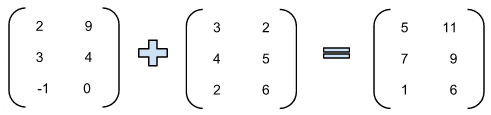
\includegraphics[width = 10cm]{Chapters/matrix-matrix-addition.png}
	\captionof{figure}{matrix addition}
\end{center}

\subsection{C++ implementation}
The C++ implementation is easy for the addition or subtraction. We can use the same function for the both operations. The pseudo code is below
\begin{lstlisting}[language=C, caption=matrix addition or subtraction in C++]
	we have m*n dimension both matrices
	if addition 
		operation = 1
	else 
		operation = -1
	for i < m; i++
		for j < n; j++
			result [i][j] = A[i][j]+(operations * B[i][j])
\end{lstlisting}
Listing 2.5, In each iteration the code will add one element of ij position of A matrix with one element of ij position of B matrix. For the subtraction we just multiply -1 with element of B matrix. And we save the result on same position in result matrix. The time complexity of this code is O($m*n$). If m is equal to n than we can say $O(n^2)$. 
\subsection{OCCA implementation}
A simple approach to compute addition or subtraction of two matrices on a GPU. The OKL pseudo code is below 
\begin{lstlisting}[language=C, caption=matrix addition or subtraction in OCCA]
	we have m*n dimension both matrices
	for o1 < m; o1+=16;@outer
			for o0 < m; o0+=16; @outer
				for y= o1; y <o1+16;y++;@inner
					for x = o0; x <o0+16;x++;@inner
						result[x][y] = A[x][y]+(operation * B[x][y])
\end{lstlisting}
Listing 2.6, The start, end and stride used in the outer and inner loops to support argument based variables and the working dimensions are resolved at run-time. Currently, working dimensions must constant across on all the inner-loops defined in outer loop. In this example x and y will work in working dimensions. In this case our working dimensions is 16. As we can see we are increment o0 and o1 by 16 and run x and y from o0 and o1 to o0+16 and o1+16. Which divide the work in group items.
\subsection{OCCA vs CPU}
\begin{center}
	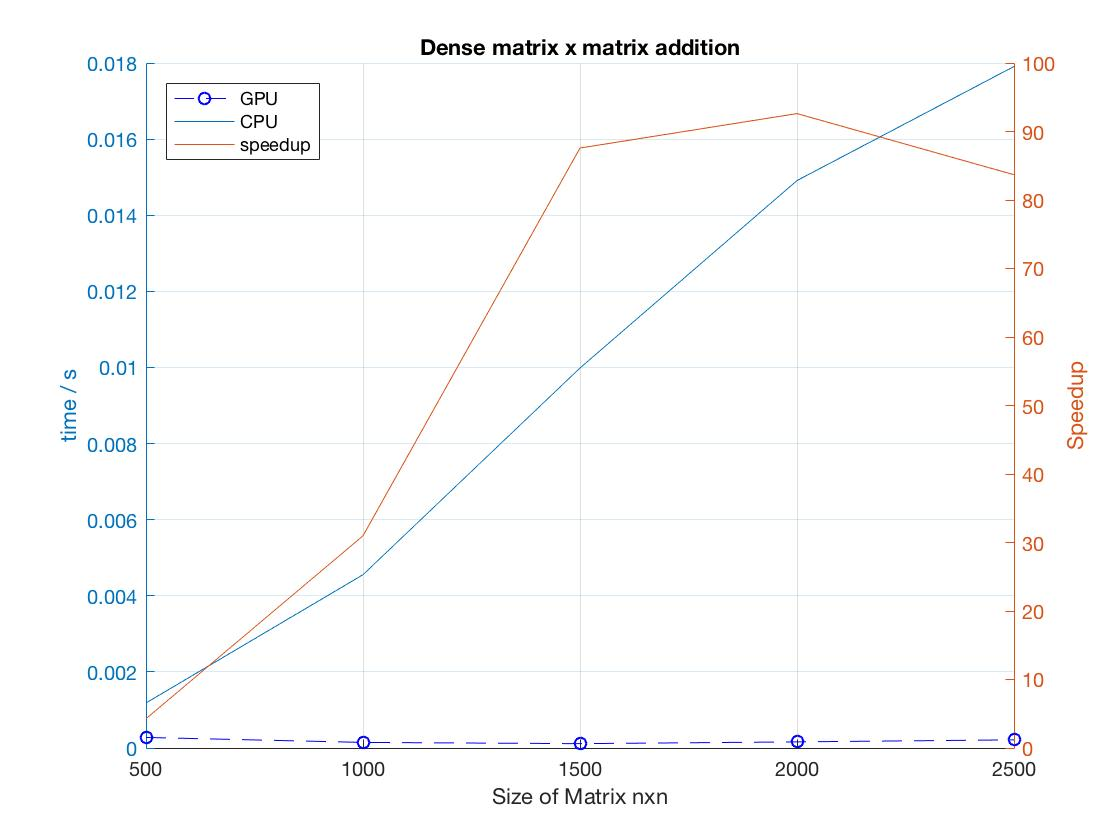
\includegraphics[width = 8cm]{Chapters/matrix_addition.jpg}
	\captionof{figure}{comparison OCCA vs CPU performance}
\end{center}
To test the performance of CPU and OCCA. We take two array of size m-by-n and compute the addition of the matrices. We use the square matrices, the dimensions of the matrices start from 500 by 500 to 2500 by 2500. The throughputs of the CPU and OCCA as shown above. We use the semiology for plotting in Matlab. If size of matrices is small than the CPU perform better than OCCA. But the large the size, the CPU gets poor performance. % Background Theory 

\chapter{Sparse Matrix}

\section{Introduction}
A sparse matrix or sparse array is a matrix in which most of the elements are zero. The number  of zero-valued elements divided by total number of elements is called sparsity of the matrix. When storing and computing sparse matrix on device it is necessary to use the efficient algorithm and data structure. Because we can store sparse matrix in significantly in less storage.
\subsection{Storing}
A matrix is typically stored as a two dimensional or one dimensional but the length of one dimensional is equal to length of (row of matrix * length of column of matrix). For m x n matrix, we require (m * n * sizeof(float)) to store the matrix.\\
But in case, Sparse matrix we need 3 vector which is equal to (3*(size of non-zero element in matrix)* sizeof(float)).
\subsection{Storing formats}
\begin{itemize}
	\item Dictionary of keys (DOK)\\
		DOK consists of a dictionary that maps (row, column)-pairs to the value of the elements. Elements that are missing from the dictionary are taken to be zero. The format is good for incrementally constructing a sparse matrix in random order, but poor for iterating over non-zero values in lexicographical order. One typically constructs a matrix in this format and then converts to another more efficient format for processing. From \ref{txt:sparsematrixformat}
	\item List of lists (LIL)\\
	LIL stores one list per row, with each entry containing the column index and the value. Typically, these entries are kept sorted by column index for faster lookup. This is another format good for incremental matrix construction. From \ref{txt:sparsematrixformat}
	\item Coordinate list (COO)\\
	COO stores a list of (row, column, value) tuples. Ideally, the entries are sorted first by row index and then by column index, to improve random access times. This is another format that is good for incremental matrix construction. From \ref{txt:sparsematrixformat}
	\item Compressed sparse row (CSR, CRS or Yale format)\\
	 We explained in \ref{sec:csr} . From \ref{txt:CSR}
	\item Compressed sparse column (CSC or CCS)\\
	CSC is similar to CSR except that values are read first by column, a row index is stored for each value, and column pointers are stored. For example, CSC is (val, rowInd, colPtr), where val is an array of the (top-to-bottom, then left-to-right) non-zero values of the matrix; rowInd is the row indices corresponding to the values; and, colPtr is the list of val indexes where each column starts. From \ref{txt:sparsematrixformat}
\end{itemize}

\section{Compressed Row Storage (CRS)}
\label{sec:csr}
A sparse matrix or sparse array is a matrix in which most of the elements are zero. The number  of zero-valued elements divided by total number of elements is called sparsity of the matrix. When storing and computing sparse matrix on device it is necessary to use the efficient algorithm and data structure. Because we can store sparse matrix in significantly in less storage.\\
\textbf{Introduction}\\
The Compressed Row and Column Storage formats are the most general. They make absolutely no assumptions about the sparsity structure of the matrix and they don't store any unnecessary elements. On the other hand, they are not very efficient, needing an indirect addressing step for every single scalar operation in a matrix-vector product or preconditioned solve. From \ref{txt:CSR}\\
For CRS, we create 3 vectors and size of the vectors are length of non-zero elements of matrix. They are 
\begin{itemize}
	\item Non-zero elements of the matrix
	\item column number for non-zero elements of the matrix
	\item row number for non-zero elements of the matrix
\end{itemize}
\begin{center}
	\includegraphics[width=12cm]{../sparse.png} 
	\captionof{figure}{convert sparse matrix to CSR format}
	\label{img:csrfo}
\end{center}


The \texttt{val}  (\ref{img:csrfo}) represents the non-zero values of the matrix, read first by row left to right, then by column top to bottom. The \texttt{colind} represents the column index corresponding to the values. The \texttt{rowptr} represents the indexes belonging to a row, it contains an index per row corresponding to an index in the two other vectors. It is clear that all indexes from this starting index and to the starting index of the next row will belong to the given row. The last index is the number of rows plus one, so the algorithm doesn’t have to check if we’re at the last row.


In this project, We use Compressed sparse row (CSR, CRS or Yale format) for our implementation.

\section{Sparse matrix - vector multiplication}
\subsection{Introduction}
Matrix vector multiplication has been implemented in the API for all kinds of matrices. We will focus on CSR formatted sparse matrix vector multiplication. An example CSR formatting with indexes starting from 1 would be the matrix\\

The matrix vector product  using CRS format can be expressed in the usual way:
\begin{equation}
	y_i = \sum _{j=1}^{n} a_{ij}x_j \quad    i \in [1...m]
\end{equation}

\begin{center}
	$\begin{bmatrix}
	1&0&0&3\\
	0&2&4&6\\
	0&0&0&0\\
	0&5&0&0
\end{bmatrix}$
\captionof{figure}{sparse matrix}
\end{center}

which would be represented by the CSR format vectors:\\
val =[1 3 2 4 6 5]\\
val is the non zero element in sparse matrix Figure 3.1.\\
col =[1 4 2 3 4 2]\\
col is the column number of non zero element in sparse matrix Figure 3.1.\\
row =[1 3 6 6 7]\\
row is the row number of non zero element in sparse matrix Figure 3.1.\\


We can perform multiplications between a matrix and vector when number of columns of matrix equal number of rows of vector
\subsection{C++ implementation}
The C++ implementation is the most basic implementation. The idea is below\\
\begin{lstlisting}[language=C, caption=matrix vector multiplication in C++]
	for i < size of non_zero elements; i++
		result[row[i]] += non_zero[i] * vector[col[i]]
\end{lstlisting}
Listing 3.1, in each iteration of the for loop, the code computes the product of non-zero element of sparse matrix and position of column number of sparse matrix with same row number of vector element. And store the result on row number of non-zero element in sparse matrix.
It is better for time and space complexity. The time complexity of this algorithm is O(size of non-zero elements).
\subsection{OCCA implementation}
We implemented this algorithm in OKL as follow\\
\begin{lstlisting}[language=C, caption=matrix vector multiplication in OCCA]
	for i=0; i < #row of matrix; i++; @tile(16, @outer, @inner)
		for j = row[i]; j <row[i+1];j++
			result[i] += non_zero[j] * vector[col[j]]
\end{lstlisting}
Listing 3.2, In this algorithm, (\#row of matrix) is the number of row in matrix and row is a vector which save the number or non-zero elements in each row. For example, we have 2 non zero elements in row 0 then its row[0] = 0 and row[1] = 2.
The most challenging is the sparse matrix-vector multiplication v = Au. Due to the  restriction in accessing the OCCA memory it is not efficient to use the standard compressed storage data format.

This algorithm runs number of rows multiply number of non zero element in the row. It store the element in result vector and in every iteration, it compute the product of non zero element and column number of non zero element position of vector element.

\subsection{OCCA vs CPU}
\begin{center}
	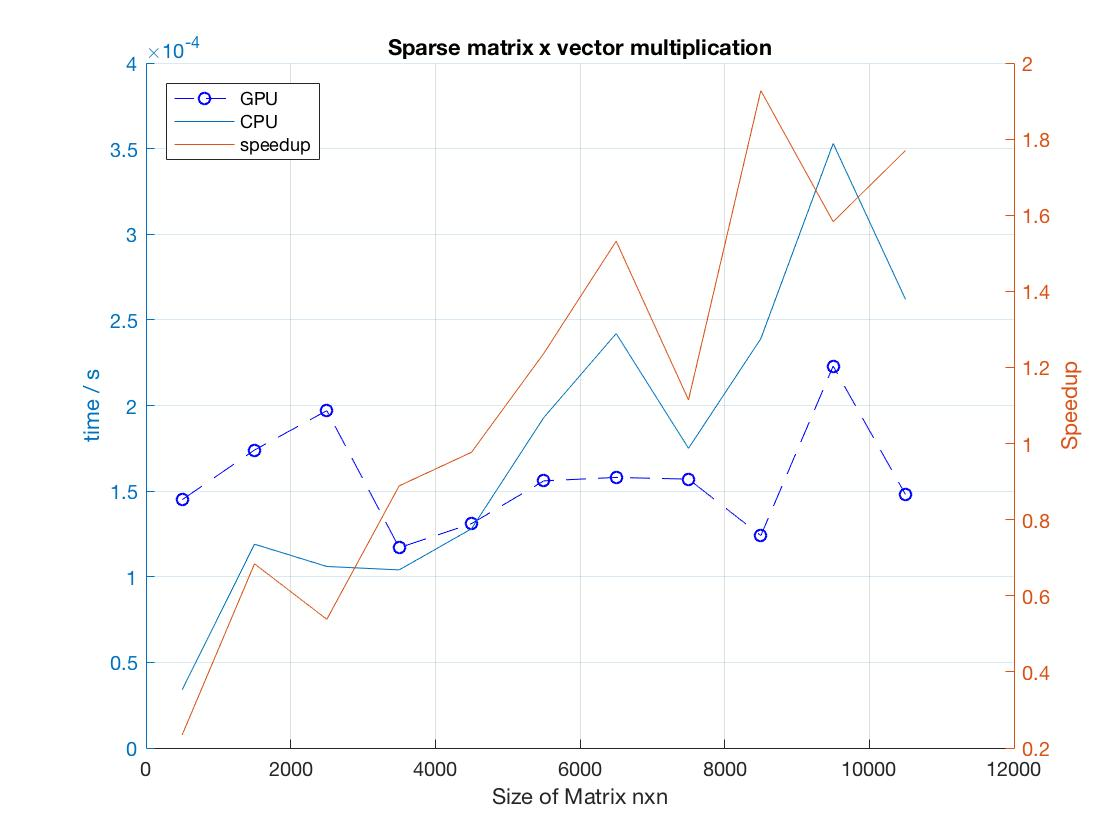
\includegraphics[width = 10cm]{Chapters/sparse_matrix_vector.jpg}
	\captionof{figure}{comparing OCCA vs CPU performance}
	\label{fig:comparisonSparse}
\end{center}
To test the performance of CPU and OCCA, we took a square sparse matrix and a vector. We save a sparse matrix in CSR format. Now we have 3 vectors, which stores non-zero elements of matrix, column number of non-zero elements in sparse matrix and row number of non-zero elements of the sparse matrix. For test cases, we use square sparse matrix. The dimension of the matrix starts from 500 by 500 to  10500 by 10500. The throughputs \ref{fig:comparisonSparse} of the CPU and OCCA as shown above. As we can see that the performance of CPU is better than OCCA, if dimension of the matrix is less than 4000. But dimension bigger than 4000, CPU performance is start fall down. And OCCA start perform better than CPU.


\section{Sparse matrix multiplication}
\subsection{Introduction}
Matrix multiplication has been implemented in the API for all kinds of matrices. We will focus on both CSR format sparse matrix multiplication. An example of CSR formatting the sparse matrix as follow\\

Let C is output matrix then mathematical formulation of the equation is described in (\ref{eq:sparsematrixmult})\\
\begin{equation}
\label{eq:sparsematrixmult}
	C_{ij}=a_{i1}b_{1j}+\cdots +a_{im}b_{mj}=\sum _{k=1}^{m}a_{ik}b_{kj}
\end{equation}
for i = 1, ..., n and j = 1, ..., p.\\
\begin{center}
	A= $\begin{bmatrix}
	1&0&0&3\\
	0&2&4&6\\
	0&0&0&0\\
	0&5&0&0
\end{bmatrix}$ B= $\begin{bmatrix}
	1&0&0&3\\
	0&2&4&6\\
	0&0&0&0\\
	0&5&0&0
\end{bmatrix}$
\captionof{figure}{A and B sparse matrix}
\end{center}

which would be represented by the vectors:\\
	A\_val =[1 3 2 4 6 5] \quad     B\_val =[1 3 2 4 6 5]\\
	A\_col =[1 4 2 3 4 2]  \quad    B\_col =[1 4 2 3 4 2]\\
	A\_row =[0 0 1 1 1 3]  \quad    B\_row =[0 0 1 1 1 3]\\


We can perform multiplications between a matrix and matrix when number of columns of matrix equal number of rows of another matrix.
\subsection{C++ implementation}
The C++ implementation pseudo code is below.
\begin{lstlisting}[language=C, caption=matrix multiplication in C++]
we use 2 vector for save the result of multiplication
int m =0;
for j < # of A non-zero elements; j++
	for k < # of B non-zero elements; k++
		check condition a_col[j] == b_row[k]
			check if the position of matrix already in array return position s
				result[s] += A_val[j]*B_val[k]
			otherwise
				result[m] = A_val[j]*B_val[k]
				position array[m] = A_row[j]* #number of column in matrix B
					 + B_col[k]
				m++
				
\end{lstlisting}
In CPU implementation, the j run from 0 to number of non-zero elements in A. Second loop k, start from 0 and end to number of the non-zero elements in B. It took j position of A\_col and compare with all the B\_row elements. Where A\_col is the column number of non-zero elements and B\_row is the row number of non-zero elements in matrix B. If we have same value on j position and k position than we have to multiply that elements and save it. After that we have to check if we already multiply and save the same row of matrix A and column of matrix B. If yes, then we have to add this in same element. If not, then we have to save result in new position of the result vector and position vector and increment the m. According to this procedure, we can save the memory because we do not need the matrix for saving the result.

\subsection{OCCA implementation}
The OCCA implementation in OKL:\\
\begin{lstlisting}[language=C, caption=matrix multiplication in OCCA]
for j < # of A non-zero elements; j++
	for o0 < # of B non-zero elements; o0++; outer
		for k = o0 k < o0+16; k++
			check condition a_col[j] == b_row[k]
					result[A_row[j]* # column in 
					matrix B + B_col[k]] = A_val[j]*B_val[k]
\end{lstlisting}
The OCCA uses the data parallelism in matrix multiplication. Except for the modified data structure for the sparse matrix storage the standard CRS matrix multiplication algorithm can be used with only minor modifications. In OKL, we just use for loops with an outer tag, which parallelised by threads (CPU) or work-groups (OCCA). We use inner tag in for-loops, which able to vectorized (CPU) or work concurrently (OCCA). The biggest problem of sparse matrix is result storage. As you can see that we are using the full length matrix for storing the result of two sparse matrix. The problem is OCCA do not define atomic operations clearly. All the working group work individually. It is not implemented till now.
\subsection{OCCA vs CPU}
\begin{center}
	\includegraphics[width = 12cm]{../matlab/sparse_matrix.jpg}
	\captionof{figure}{comparing OCCA vs CPU performance}
\end{center}
To test the performance of CPU and OCCA, we took two square sparse matrix. We save each sparse matrix in 3 vectors in CSR format. Now we have 6 vector for sparse matrices, which stores non-zero elements of matrix, column number of non-zero elements in sparse matrix and row number of non-zero elements of the sparse matrix. For test cases, we use square sparse matrices. The dimensions of the matrices start from 2000 by 2000 to  14000 by 14000. We use the semiology for plotting in Matlab. The throughputs of the CPU and OCCA as shown above. As we can see that the performance of CPU is better than OCCA, if dimension of the matrix is less than 10000. But dimension bigger than 10000, CPU performance is starting fall down. And OCCA start perform better than CPU. CPU rise too fast after 12000. Because when we increase the matrix size it also increase the non-zero elements in matrix.

\section{Sparse matrix - matrix addition \& subtraction}
\subsection{Introduction}
Sparse matrix addition or subtraction is not difficult. Firstly, we have to save both matrix in CSR formats.\\
Let C is output matrix then mathematical formulation of the equation is\\
\begin{equation}
	C_{ij}=a_{ij} \pm b_{ij}
\end{equation}

for i = 1, ..., n and j = 1, ..., p.\\
That is, the entry $C_{ij}$ is the sum or subtracion of the $i^{th}$ row and $j^{th}$ of A and the $i^{th}$ row and $j^{th}$ of B.\\
\begin{center}
	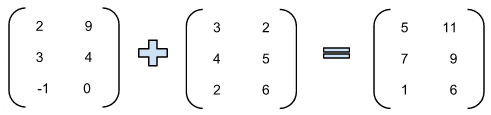
\includegraphics[width=10cm]{Chapters/matrix-matrix-addition} 
	\captionof{figure}{matrix addition}
\end{center}
	A\_val =[1 3 2 4 6 5] \quad     B\_val =[1 3 2 4 6 5]\\
	A\_col =[1 4 2 3 4 2]  \quad    B\_col =[1 4 2 3 4 2]\\
	A\_row =[0 0 1 1 1 3]  \quad    B\_row =[0 0 1 1 1 3]\\
	Normally, we have to add $j^{th}$ position of element of matrix A in $j^{th}$ position of element of matrix B and save it on $j^{th}$ position in result matrix.\\
	We have to be same dimensional matrices for addition or subtraction of matrices.
\subsection{CPU implementation}
CPU implementation addition (or subtraction) operation for sparse matrix with CSR format is described in the pseudocode:
\begin{lstlisting}[language=C, caption=matrix addition (or subtraction) in C++]
we have two vector of #non zero elements in A + #non zero elements in B

# copy A_non_zero elements to result
for i < #non zero elements in A; i++
	result[i] = A_non Zero [i]
	position[i] = A_row[i] * #number of column matrix A + A_col_number[i]
# copy B_non_zero elements to result
for i < #non zero elements in B;i++
	result[i+#non zero elements in A] = B_non Zero [i]
	position[i+#non zero elements in A] = B_row[i] * #number of column matrix B + B_col_number[i]
# checking if matrix a and matrix b have non zero element on same position
for i < #non zero elements in A + #non zero elements in B-1;i++
	for j < #non zero elements in A + #non zero elements in B;j++
		check condition i !=j && i<j
		check condition position[i] == position[j]
			result[i] += result[j]
			result[j] = 0;
			position[j] = 0;




\end{lstlisting}
As we can see, we have two vectors for save the output result and position. In result vector, we save the addition or subtraction of matrix A elements with matrix B elements. Position vector, we save the position of the result element. In this algorithm we are firstly save all the non zero element of matrix A and after we save all the non zero element of matrix B. As same as, we save position of all the non zero elements A and B in vector position. And in the end we just walk through the result vector and position vector. When we have duplicate element in vector position, we add that position element of result vector to the duplicate position element and make it zero and also remove element from the position vector make it zero.
\subsection{OCCA implementation}
The OCCA implementation for sparse matrix addition or subtraction pseudocode is below:
\begin{lstlisting}[language=C, caption=matrix addition (or subtraction) in OCCA]
we have two vector of #non zero elements in A + #non zero elements in B
for i < #non zero elements in A;i++;@tile(16, @outer, @inner)
	result[i] = A_non Zero [i]
	position[i] = A_row[i] * #number of column matrix A + A_col_number[i]
for i < #non zero elements in B;i++;@tile(16, @outer, @inner)
	result[i+#non zero elements in A] = B_non Zero [i]
	position[i+#non zero elements in A] = B_row[i] * #number of column matrix                                    B + B_col_number[i]
for o1 < #non zero elements in A + #non zero elements in B-17;o1++;@outer
	for o0 < #non zero elements in A + #non zero elements in B;o0++;@outer
		for i = o1; i < o1+16;i++;@inner
	for j = o0; j < o1+16;j++;@inner
		check condition i !=j && i<j
		check condition position[i] == position[j]
			result[i] += result[j]
			result[j] = 0;
			position[j] = 0;
\end{lstlisting}
Both plus and minus share the same code. I have only presented plus operation. While it's called matrix addition, it can work for all data types, but it only applies to the values. That is, in the sparse, we only store values for given coordinates, but we can still add a sparse matrix to a sparse matrix.\\
In OCCA implementation is similar to the CPU implementation, but in first two loops we add fourth clause tile in for-loop that indicating the type of parallelism to be take by the for-loop. After that next two loops we use the outer1 and outer0 in for-loops, which parallelised by threads (CPU) or working-groups (OCCA). Afterward we have for-loops with the inner tag, which able to be vectorized (CPU) or or work concurrently (OCCA). We have to check the condition i != j because it will add the same position value again and again. Now we have to check the duplicate element in position vector and add the same position result element. And make it zero in result vector and position vector. 
\subsection{OCCA vs CPU}
\begin{center}
	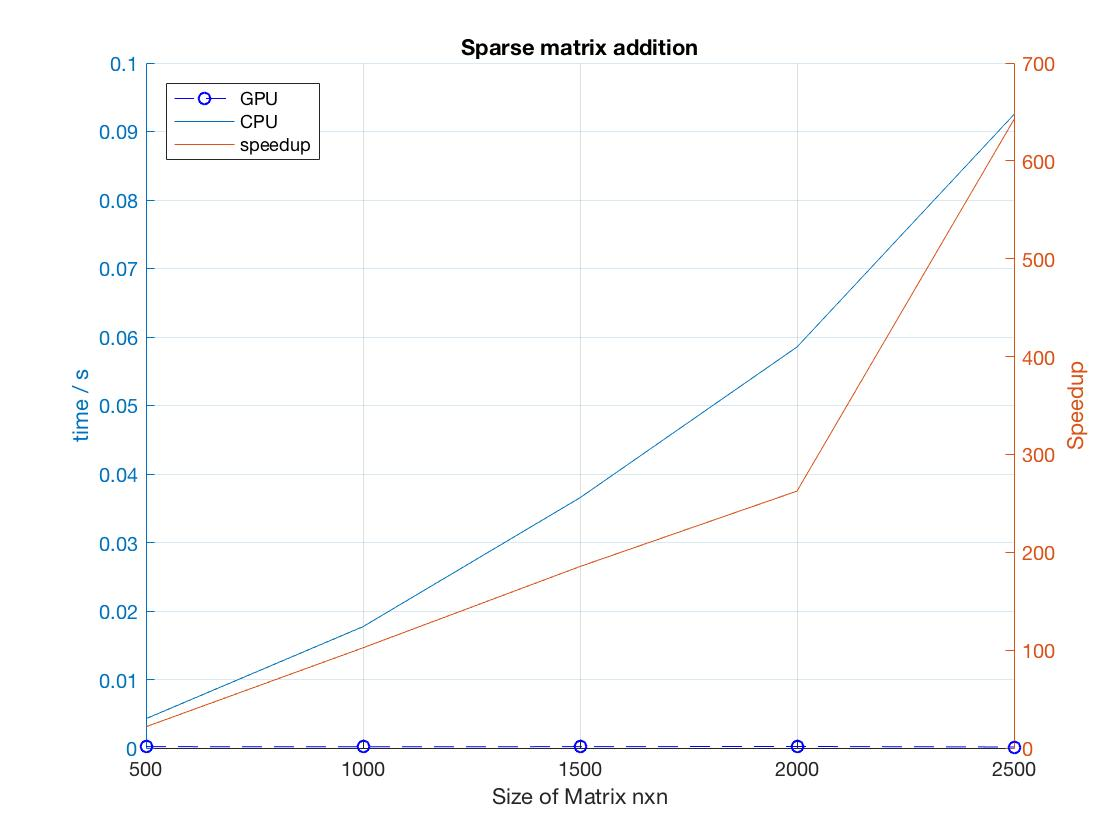
\includegraphics[width = 12cm]{Chapters/sparse_matrix_addition.jpg}
	\captionof{figure}{compare OCCA vs CPU performance }
\end{center}
As we can be see, the performance of CPU is not very good as expected. We use the two sparse matrices and convert it in the CSR format. The dimension of the matrix starts from 500 by 500 to  2500 by 2500. We use the semiology for plotting in Matlab. The throughputs of the CPU and OCCA as shown above. As we can see, the performance of OCCA is better than CPU, if we choose matrices size bigger.







 % Experimental Setup

%\setcounter{secnumdepth}{-1}
    \chapter{Dot product}
    \section{Introduction}
    The dot product or scalar product is an algebraic operation that takes two equal length sequence of numbers and return a single number.\\
 The dot product of two vectors a = [a1, a2, ..., an] and b = [b1, b2, ..., bn] is defined as:\\
 \begin{equation}
 	\mathbf {a} \cdot \mathbf {b} =\sum_{i=1}^{n}a_{i}b_{i}=a_{1}b_{1}+a_{2}b_{2}+\cdots +a_{n}b_{n}
 \end{equation}
%$\mathbf {a} \cdot \mathbf {b} =\sum_{i=1}^{n}a_{i}b_{i}=a_{1}b_{1}+a_{2}b_{2}+\cdots +a_{n}b_{n}$\\
where $\sum$ denotes summation and n is the dimension of the vector space.\\
\begin{equation}
	\begin{bmatrix}1&3&-5\end{bmatrix}
    	\begin{bmatrix}4\\-2\\-1\end{bmatrix}= 1*4+3*(-2)+(-5)*(-1) = 3.
\end{equation}
%    	$\begin{bmatrix}1&3&-5\end{bmatrix}
%    	\begin{bmatrix}4\\-2\\-1\end{bmatrix}= 1*4+3*(-2)+(-5)*(-1) = 3.$\\
	For dot product, we have to same length of both vectors.
    \section{CPU implementation}
    The CPU implementation is below:\\
    \begin{lstlisting}[language=C, caption=vector dot product in C++]
    	for i < size of vector;i++
    		result += vector1[i] * vector2[i]
    \end{lstlisting}
    As we can see, It is simple to implement in CPU. We walk through the vector1 and vector2 and  multiply the same position elements of both vectors and add result in previous result.
 	\section{OCCA implementation / Reduction}
 	Kernel implementation of dot product is below.
 	\begin{lstlisting}[language=C, caption=vector dot product in OCCA]
 for (int group = 0; group < ((entries + block - 1) / block); ++group; @outer) {
        shared float s_vec[256];
        for (int item = 0; item < block; ++item; @inner) {
            if ((group * block + item) < entries) {
                s_vec[item] = vec[group * block + item] * vec2[group * block + item];
            } else {
                s_vec[item] = 0;
            }
        }
		for (int alive = ((block + 1) / 2); 0 < alive; alive /= 2) {
            for (int item = 0; item < block; ++item; @inner) {
                if (item < alive) {
                    s_vec[item] += s_vec[item + alive];
                }
            }
            for (int item = 0; item < block; ++item; @inner) {
                if (item == 0) {
                    blockSum[group] = s_vec[0];
                }
            }
        }
    }
 	\end{lstlisting}
 	We implement partial reduction of of vector using loop tiles of size block. In this case block is 256. As we can see firstly we save elements multiplication in shared memory. Now it will produce a vector of length block. Now in next loop it alive point to middle of the vector and item point 0 of vector. we add the elements of the vector and save it on position 0. In next loop, we just copy result to blocksum. 
 	\section{GPU vs CPU}
 	As we can estimate GPU will more expensive than CPU. Because in GPU firstly we have to copy the multiplication to the  shared memory. After that we start the partial reduction . And we know that memory transfer in GPU is more expensive than CPU. Another reason is that we implemented with partial reduction in GPU, but in CPU we are implement without reduction. 
 	
 % Experiment 2

\chapter{Gaussian elimination}

\section{Introduction}
Gaussian elimination (also known as row reduction) is an algorithm for solving systems of linear equations. It is usually understood as a sequence of operations performed on the corresponding matrix of coefficients. \\
The fundamental idea is to add multiples of one equation to the others in order to eliminate a variable and to continue this process until only one variable is left. Once this final variable is determined, its value is substituted back into the other equations in order to evaluate the remaining unknowns. This method, characterized by step$-$by$-$step  elimination of the variables, is called Gaussian elimination.\\
$\begin{bmatrix}
1&3& \\
2&1&				
\end{bmatrix}$
$\begin{bmatrix}
x \\
y				
\end{bmatrix}$
=
$\begin{bmatrix}
3 \\
5				
\end{bmatrix}$\\

$\begin{matrix}
1x+3y = 3 \\
2x+1y = 5				
\end{matrix}$\\

Multiply row 1 by 2 and subtract from row 2 \\
$\begin{matrix}
1x+3y = 3 \\
5y = 1				
\end{matrix}$\\
$\begin{matrix}
x = 12/5 \\
y = 1/5				
\end{matrix}$
\section{C++ implementation}
The C++ implementation as below:
\begin{lstlisting}[language=C, caption=Gauss elimination in C++]
	void Gauss_elmination_cpu(float a[], float d[], int n) {
	int i, j, k, temp;
	//********* Forward elimination process**************//
	for (int i = 0; i < n - 1; i++) {
		for (int k = i + 1; k < n; k++) {
			float c = a[k * (n + 1) + i] / a[i * (n + 1) + i];
			for (int j = i; j <= n; j++) {
				a[k * (n + 1) + j] = a[k * (n + 1) + j] - (c * a[i * (n + 1) + j]);
			}
		}
	}
    //***************** Backward Substitution method****************//
	for (i = n - 1; i >= 0; i--){
		d[i] = a[i * (n + 1) + n];
		for (int j = i + 1; j < n; j++) {
			if (j != i) {
				d[i] = d[i] - a[i * (n + 1) + j] * d[j];
			}
		}
		d[i] = d[i] / a[i * (n + 1) + i];
	}
}
\end{lstlisting}
\textbf{Forward elimination:} reduction to row echelon form. Using it one can tell whether there are no solutions, or unique solution, or infinitely many solutions.\\
\textbf{Back substitution:} further reduction to reduced row echelon form.\\
In this code, We have i is the row number of matrix and k is walk through all the row which are below the $i^{th}$  row. We have variable c which store the difference of $i^{th}$ row, $i^{th}$ column and $k^{th}$ row, $i^{th}$  column. And j walk through the element of $i^{th}$ and $k^{th}$ row. After finishing this method, We have upper triangular matrix.\\
Which we can solve by backward substitution method. We walk from down to up. We got the value and we use it for solve next value.

\section{OCCA implementation}
Kernel implementation of Guass Elimination is below.
\begin{lstlisting}[language=C, caption=Gauss elimination in OCCA]
    //********* Forward elimination process**************//
    for (int k =i+1; k<n; k++; @tile(16, @outer, @inner)) {
        float c = a[k*(n+1)+i]/a[i*(n+1)+i];
        for (int j=0; j<= n; j++) {
            a[k*(n+1)+j]=a[k*(n+1)+j]-(c*a[i*(n+1)+j]);
        }
    }
}
//***************** Backward Substitution method****************//
  for (int k =0; k < 1; k++; @tile(16, @outer, @inner)) {
        d[i] = a[i*(n+1)+n];
    	for (int j =0; j <n; j++) {
            if (j > i) {
                d[i] = d[i] - (a[i*(n+1)+j] * d[j]);
            }
        }
    	d[i] = d[i]/a[i*(n+1)+i];
    }
}
\end{lstlisting}

In OCCA, We implement the forward substitution and backward substitution method separately. Currently, working dimensions must constant across on all the inner-loops defined in outer loop (@tile(16, @outer, @inner)). In this example k will work in working dimensions. In this case our working dimensions is 16. But the implementation idea is same as CPU implementation.

\section{OCCA vs CPU}
\begin{center}
	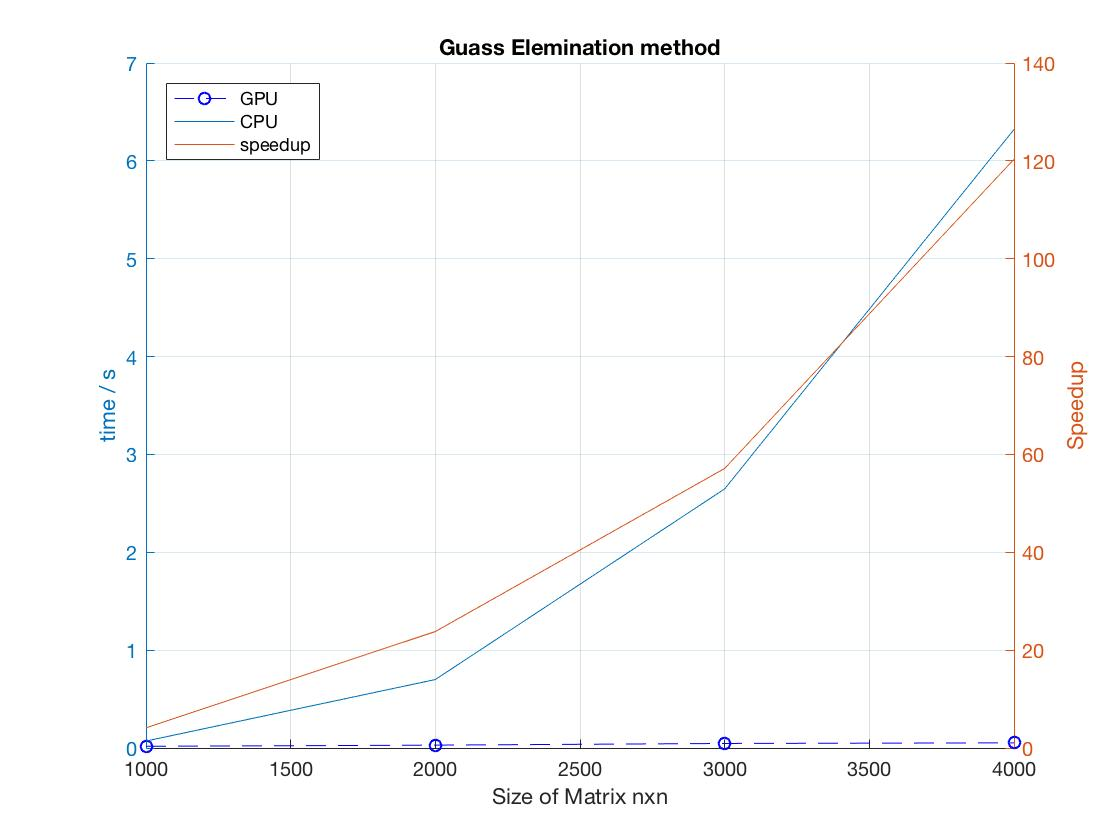
\includegraphics[width = 12cm]{Chapters/guass_elimination.jpg}
	\captionof{figure}{compare OCCA vs CPU performance }
\end{center}

As we can see CPU will more expensive than OCCA. We measure the length of matrix from 500X500 to 4000X4000. And GPU always take time near 0.xxx and CPU takes more time according to length of matrix. According to this conclusion, We can say that OCCA is better than CPU. 


\chapter{Jacobi method}
\section{Introduction}
Jacobi method is an iterative solver used for approximating the solution of diagonally dominant system of linear equations. 
The Jacobi method is easily derived by examining each of the n equations in the linear system Ax = b in isolation. If in the $i^{th}$ equation \\
\begin{equation}
	\sum^n_{j=1}a_{i,j}x_j = b_i
\end{equation}
We solve for the value of $x_i$ while assuming the other entries of x remain fixed, We obtain\\
\begin{equation}
	x_i = (b_i - \sum_{j\neq i}a_{i,j}x_j)/a_{i,i}
\end{equation}
This suggests an iterative method defined by \\
\begin{equation}
	x_i^{(k)} = (b_i - \sum_{j\neq i}a_{i,j}x_j^{(k-1})/a_{i,i}
\end{equation}

Which is the Jacobi method.

\section{C++ implementation}
The C++ implementation as below:
\begin{lstlisting}[language=C, caption=Jacobi method in C++]
	for (int k = 0; k < num_iter; k++) {
		for (int i = 0; i < n; i++ ) {
			float sum = 0;
			for (int j = 0; j < n; j++ ) {
				if ( j != i ) {
					sum += (a[i * (n + 1)+ j] * x[j]);
				}
			}
            x_new[i] = ((a[i * (n + 1) + n]) - sum ) / a[i + i * (n + 1)];
        }
		for (int i = 0; i < n; i++) {
			x[i] = x_new[i];
        }
	}
\end{lstlisting}
This is Jacobi method, Where first loop is count the number of iteration and another loop i,j are start from 0 to n which is the size of the matrix nXn. x is the initial guess vector and x\_new is result vector. And in the last loop, We copy the x\_new to x. It run again and again till k is not equal or bigger than number of iteration.
\section{OCCA implementation}
The OCCA implementation as below:
\begin{lstlisting}[language=C, caption=Jacobi method in OCCA]
	for (int i = 0; i < n; i++; @tile(16, @outer, @inner) ) {
		x_new[i] = a[i * (n + 1) + n];
		float sum =0;
		for (int j = 0; j < n; j++ ) {
			if ( j != i ) {
				sum += a[i + j * (n + 1)] * x[j];
            }
        }
         x_new[i] = ((a[i * (n + 1) + n]) - sum ) / a[i + i * (n + 1)];
        }
        for (int i = 0; i < n; i++; @tile(16, @outer, @inner){
    		x[i] = x_new[i];
    }
\end{lstlisting}
This is OCCA implementation of Jacobi method. It is same as CPU implementation but here we are using the fourth value for for loop. It is @tile(16, @outer, @inner), the tile tag, tiling for-loops as one and two dimensional sets of inner/outer loops. The tile(16) assign the working dimension. In this example it assign the working dimension is 16. 
\section{OCCA vs CPU}
\begin{center}
	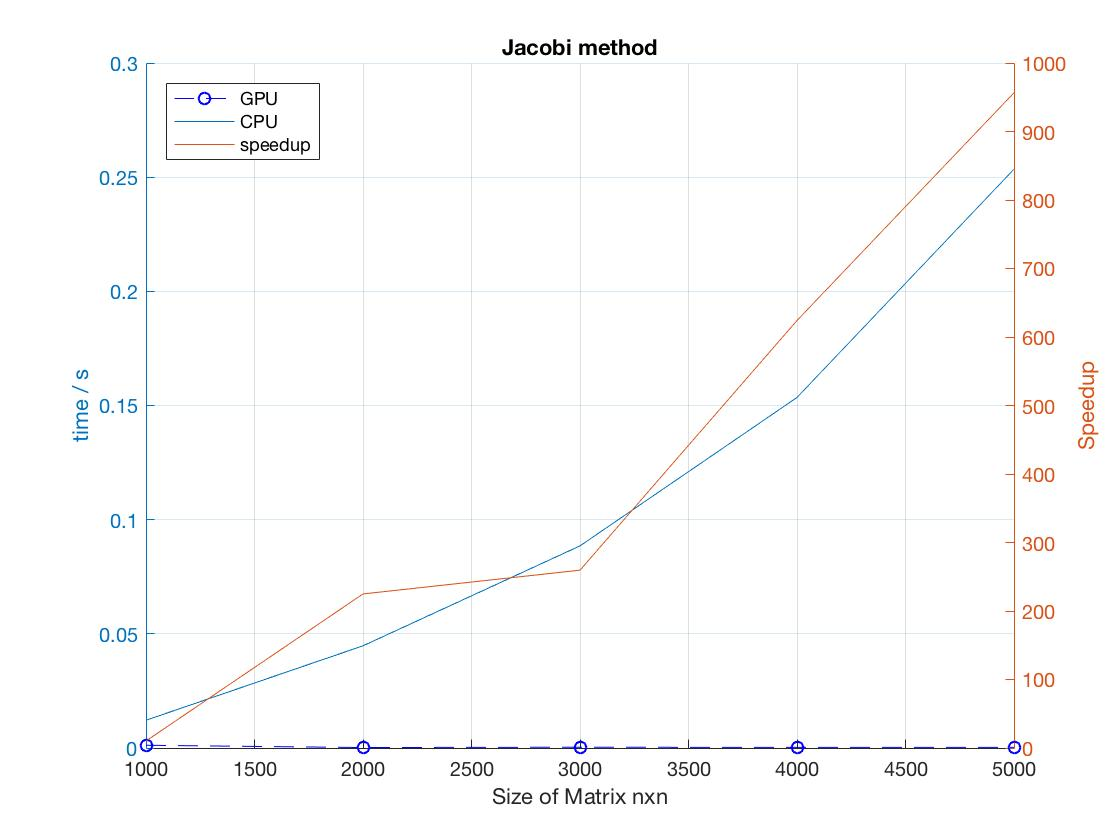
\includegraphics[width = 12cm]{Chapters/jacobi_method.jpg}
	\captionof{figure}{compare OCCA vs CPU performance }
\end{center}

For Jacobi method, OCCA is better than CPU. We can compare according to our results. We compare the matrix size from 1000X1000 to 5000X5000. In this size matrix, OCCA finish the program in 0.xxx time and CPU take time more than 0.2xx and it increase strictly according to size of the matrix.  % Experiment 2

%\setcounter{secnumdepth}{-1}
    \chapter{Multigrid Method}
    \section{Introduction}
    Multigrid (MG) methods in numerical analysis are algorithms for solving differential equations using a hierarchy of discretizations. They are an example of a class of techniques called multiresolution methods, very useful in problems exhibiting multiple scales of behavior.\\
     The main idea of multigrid is to accelerate the convergence of a basic iterative method (known as relaxation, which generally reduces short-wavelength error) by a global correction of the fine grid solution approximation from time to time, accomplished by solving a coarse problem. From \ref{txt:multigrid}
     
%     \subsubsection{Solution Methods} 
%To solve the systems of linear equations we are using this methods:\\
%• Direct\\
%– Gaussian elimination \\
%• Iterative\\
%– Jacobi\\

\section{Multigrid pseudo-code}

The main structure of a MultiGrid algorithm should be describe by following sequence of operations \ref{eq:main}

\begin{align}
	v^h = MultiGrid(A^h, v^h,f^h,\alpha_1, \alpha_2)
	\label{eq:main} 
\end{align}
\begin{equation}
	Relex\quad \alpha_1 \quad times\quad on\quad A^h u^h = f^h \quad on \quad  \Omega^h \quad with \quad arbitrary \quad initial \quad guess \quad v^h
	\label{eq:relax}
\end{equation}
\begin{equation}
\label{eq:computeB}
	compute \quad residual \quad on \quad  fine \quad  grid \quad r^h = f^h - A^hv^h
\end{equation}
\begin{equation}
\label{eq:computeB2h}
	reduce \quad residual \quad on \quad  coarse \quad  grid \quad r^{2h} = I^{2h}_h r^h
\end{equation}
\begin{equation}
	reduce \quad matrix \quad on \quad  coarse \quad  grid \quad A^{2h} = I^{h}_{2h} A^h I_{h}^{2h}
\end{equation}
\begin{equation}
\label{eq:recursivecall}
	Recursive\quad call\quad to\quad MultiGrid \  to \  solve \quad A^{2h}e^{2h} = r^{2h} \quad on \quad \Omega^{2h}
\end{equation}
\begin{equation}
\label{eq:addx}
	correct \quad fine \quad grid \quad solution \quad v^h = v^h + I_{2h}^he^{2h}
\end{equation}
\begin{equation}
	Relex\quad \alpha_2 \quad times\quad on\quad A^h u^h = f^h \quad on \quad  \Omega^h \quad with \quad v^h
\end{equation}

In this procedure, we relax  $\alpha_1$ times the system of equation $A^h u^h = f^h$ with the given initial guess $v^h$. In this project we use the Jacobi method. We  compute the residuals $r^h$ with the new $v^h$. After that, we  use the reduction operator on $r^h$. We  reduce the matrix $A^h$ by applying the reduction and interpolation operators. Which return $A^{2h}$. Now, We use the recusrion with our new system $A^{2h}e^{2h} = r^{2h}$ to solve system on coarse grid $\Omega^{2h}$. And after that we correct the solution on fine grid $v^h$ by using the correction $e^{2h}$. And finally, we relax with $\alpha_2$ times our $A^h u^h = f^h$ with the initial guess $v^h$.
\section{Multigrid mehtod Dense matrix}

\subsection{Introduction}

In the multi-grid method, We use the Gauss elimination method as exact solver, Jacobi method for relaxation. Some specific functions for matrix interpolation, matrix reduction, vector interpolation. The main idea is \\
\begin{lstlisting}[language=C, caption=multigrid method idea]
	multi-grid method(a, b, x, recursion)
		if (recursion == 0)
			gauss-elimination method(a, b, x)
			return 
		jacobi method(a, b, x, 10)
		
		\\reduction of vector b
		b2h = Reduction (b - a*x)
		
		\\ initialize 
		x2h = 0
		
		\\ compute a2h, R = reduction matrix, I = interpolation matrix
		a2h = R *  a * I
		
		multi-grid method(a2h, b2h, x2h, recursion-1)
		
		xh = interpolation x2h
		
		x = x + xh
		
		jacobi method(a, b, x, 10)
		
\end{lstlisting}
 
With the reduction, We decrease the size of the vector. For example if we have a vector of size n, after reduction we obtain a new vector of size n/2. We call the multi-grid method again with the reduced  $A$, $b$ and $x$. And we repeat this process until the recursion counter is equal to 0; and when it is 0, It calls the Gauss elimination method to solve the given system by stopping the recursive calls.
 

\subsection{C++ implementation}

The C++ implementation as below:\\
\begin{lstlisting}[language=C, caption=Multigrid method in C++]
	if (recursion == 0) {

        Gauss_elmination_cpu(a, b, x, row);
        return ;
    }
    float *x_new2 = new float[row];

    init_zero(x_new2, row);
    jacobi_method_cpu(a, x, b, x_new2, row, alpha);

    float *b2h = new float[row / 2];
    float *res1 = new float[row];
    float *x_new2h = new float[row];
    float *a2h = new float[(row / 2) * (row / 2)];

    init_zero(b2h, row / 2);
    init_zero(res1, row);
    init_zero(x_new2h, row);
    init_zero(a2h, (row / 2) * (row / 2));

    matrix_x_vector(row, row, x, a, x_new2h);

    add_sub_vector(b, x_new2h, res1, row,  -1);

    reduction_vector(res1, (row / 2), b2h);

    init_zero(x_new2h, row);

    interpolation_reduction_matrix(a, row, a2h);

    if (row / 2 <= 0) {
        cout << "error" << endl;
        return;
    }
    multigrid_method(a2h, x_new2h, b2h, recursion - 1, row / 2, alpha);

    float * res_int = new float[(row * 2) + 1];
    init_zero(res_int, (row * 2) + 1);

    reduction_interpolation_vector(x_new2h, row, res_int);
    add_sub_vector(x, res_int, x, row,  1);

    jacobi_method_cpu(a, x, b, x_new2, row, alpha);
\end{lstlisting}

In CPU, It is the same implementation as I describe above. Firstly, We check if the recursion is
0 or not. If yes, we call the Gauss elimination method and stop the recursion. If not,
We call to Jacobi method alpha times. We calculate the $b_h^{2h}$,$x_h^{2h}$  and $a_h^{2h}$. Size of $x_h^{2h}$ is half of size $x_{2h}^h$. And we call multigrid method recusively with the $b_h^{2h}$,$x_h^{2h}$  and $a_h^{2h}$. And subtract 1 from recursion. After recursion call, We convert $x_h^{2h}$ to $x_{2h}^h$ and add in x. In last, We call Jacabi method again alpha time. 


\subsection{OCCA implemintation}
The OCCA implementation as below:\\
\begin{lstlisting}[language=C, caption=multigrid method in OCCA]
	if (recursion == 0) {
        gauss_elmination_call_gpu(row, o_a, o_b, o_x, device);
        return;
    }
    occa::memory o_d, o_b2h, o_x2h, o_a2h, o_res, o_res_result2h;
    // Allocate memory on the device

    o_d  = device.malloc(row * sizeof(float));
    o_b2h  = device.malloc((row / 2) * sizeof(float));
    o_x2h  = device.malloc(row * sizeof(float));
    o_res  = device.malloc(row * sizeof(float));
    o_a2h  = device.malloc((row / 2) * (row / 2) * sizeof(float));
    o_res_result2h  = device.malloc(((row * 2) + 1) * sizeof(float));

    jacobi_method_call_gpu(row, o_a, o_b, o_x, o_d, device, alpha);

    dense_Matrix_Vector_Multiplication_call_gpu(row, o_a, o_x, o_res, device);

    add_sub_call_gpu(row, o_b, o_res, o_res, device, -1);

    relaxation_reduction_vector(row / 2, o_res, o_b2h, device);

    reduction_interpolation_reduction_matrix_call_gpu(row, o_a, o_a2h, device);

    if (row / 2 <= 0) {
        cout << "error" << endl;
        return;
    }

    multigrid_method_gpu(row / 2, o_a2h, o_b2h, o_x2h, device, recursion - 1, alpha);

    relaxation_interpolation_vector_call_gpu(row, o_x2h, o_res_result2h, device);

    add_sub_call_gpu(row, o_x, o_res_result2h, o_x, device, 1);

    jacobi_method_call_gpu(row, o_a, o_b, o_x, o_d, device, alpha);
\end{lstlisting}

It has same idea like CPU implementation, We just make all calculation on OCCA. And we described before Gauss elimination and Jacobi method in OCCA. 

\subsection{OCCA vs CPU}
\begin{center}
	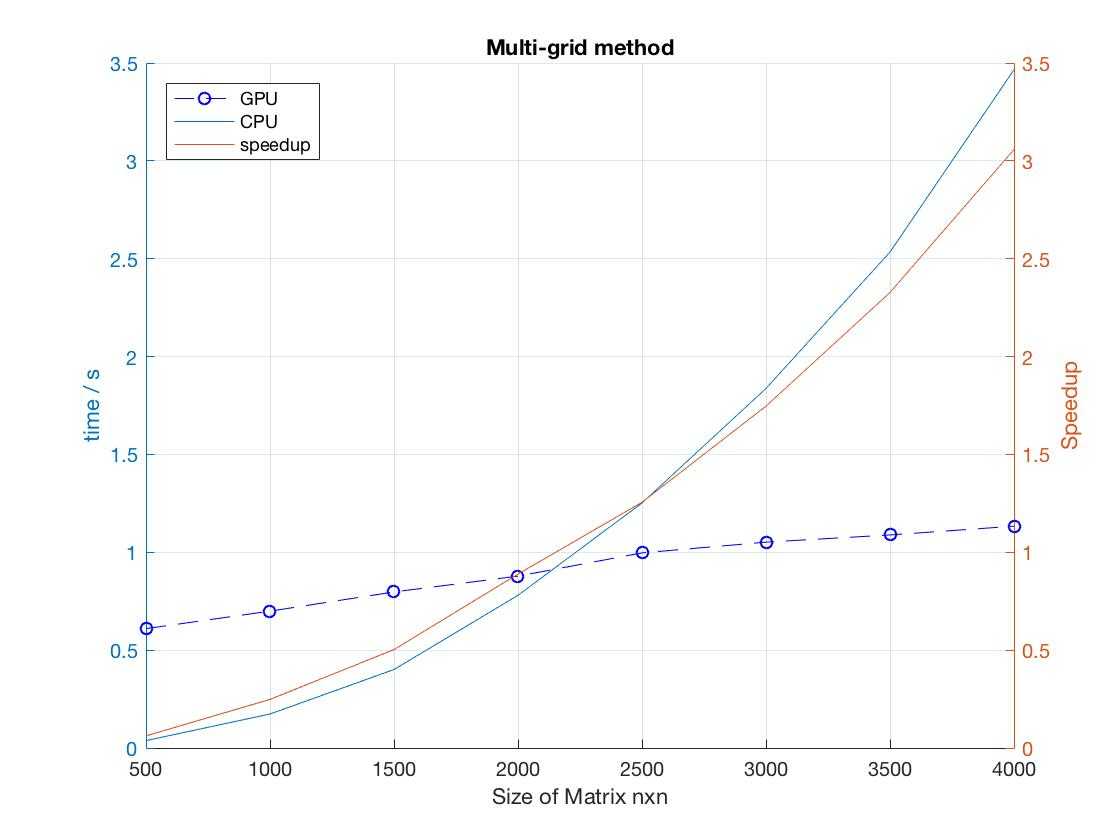
\includegraphics[width = 12cm]{Chapters/multigrid.jpg}
	\captionof{figure}{compare OCCA vs CPU performance}
	\label{img:dmatrix}
\end{center}



In this graph \ref{img:dmatrix} we observe that if the matrix size is small CPU is better than OCCA with GPU. And according to size of matrix, the CPU time increase faster also. But OCCA is increase very slightly. In my opinion, OCCA is much better if the  matrix size is large and OCCA with GPU is faster than CPU. 

\subsection{Numerical analysis of results}
\begin{center}
	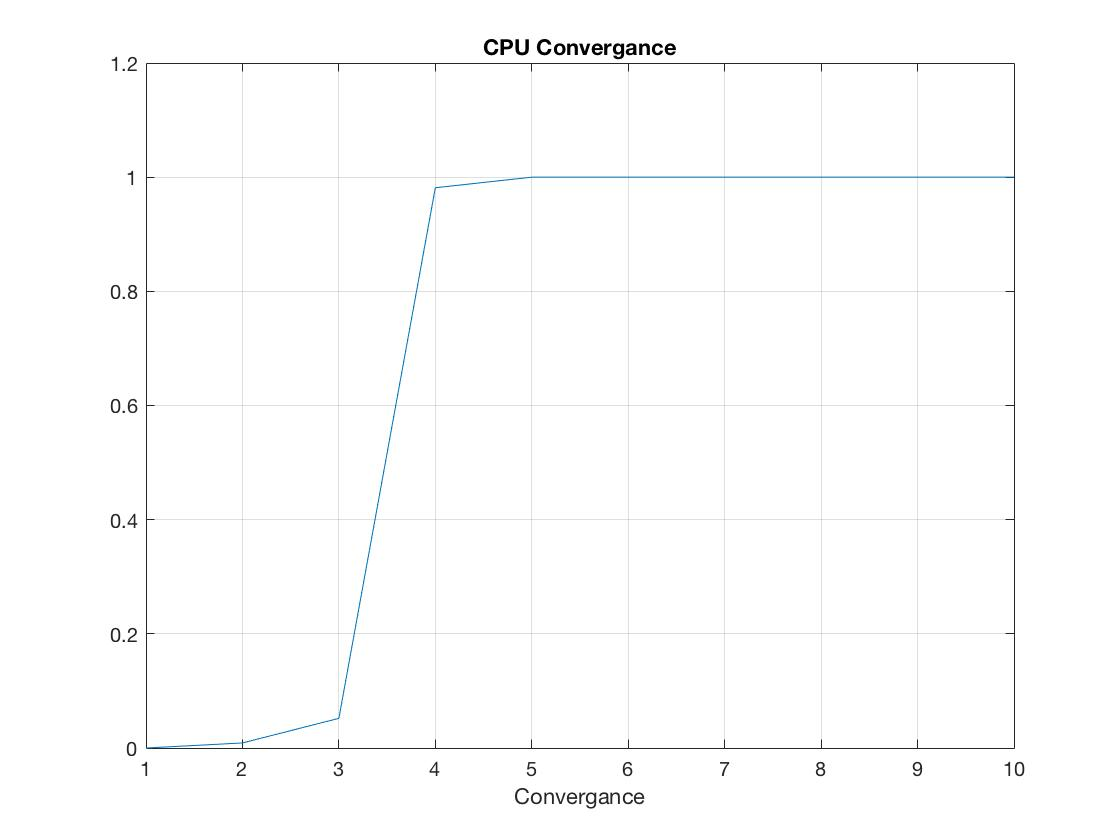
\includegraphics[width = 12cm]{Chapters/cpu_convergence_dense}
	\captionof{figure}{Convergence rate}
	\label{img:convergenceDense}
\end{center}

This convergence rate \ref{img:convergenceDense}, which refer to SPD matrix 2000 by 2000. We have used 32 bit plotting point. In 4s Multigrid step, it converge to solution. 
\section{Multigrid mehtod sparse matrix}
 

\subsection{C++ implementation}

The C++ implementation as below:\\
\begin{lstlisting}[language=C, caption=multigrid method in C++]
	void multigrid_method_sparse_matrix(float a_non_zero[], int a_col_number[], int a_row[], float x[], float b[], int recursion, int row, int alpha, int size_a) {

    if (recursion == 0 || row / 2 < 3 ) {
        int *point = new int[size_a];
        float *aa  = new float [row * row];
        for (int i = 0; i < size_a; i++) {
            point[i] = a_col_number[i] * row + a_row[i];
        }

        vectorToMatrix(row, row, size_a, a_non_zero, aa, point);

        Gauss_elmination_cpu(aa, b, x, row);

        delete [] point;
        delete [] aa;

        return ;
    }


    float *x_new2 = new float[row];
    init_zero(x_new2, row);

    jacobi_method_cpu_sparse_matrix(a_non_zero, a_col_number, a_row, b, x, x_new2, row, alpha, size_a);


    float *b2h = new float[row / 2];
    float *res1 = new float[row];
    float *x_new2h = new float[row];

    init_zero(b2h, row / 2);
    init_zero(res1, row);
    init_zero(x_new2h, row);

    sparse_matrix_x_vector(row, size_a, x, a_row, a_col_number, a_non_zero, x_new2h);
    add_sub_vector(b, x_new2h, res1, row,  -1);
    reduction_vector_sparse(res1, row, b2h);

    init_zero(x_new2h, row);

    int size_non = (size_a + row) * 3;

    float *a2h = new float[size_non];
    int *a2h_row = new int[size_non];
    int *a2h_col = new int[size_non];

    init_zero(a2h, size_non);
    init_zero(a2h_row, size_non);
    init_zero(a2h_col, size_non);


    size_non = interpolation_reduction_matrix_sparse_matrix(a_non_zero, a_col_number, a_row, size_a, row, a2h, a2h_row, a2h_col);

    multigrid_method_sparse_matrix(a2h, a2h_col, a2h_row, x_new2h, b2h, recursion - 1, row / 2, alpha, size_non);

    float * res_int = new float[(row * 2) + 1];

    init_zero(res_int, (row * 2) + 1);

    reduction_interpolation_vector(x_new2h, row, res_int);

    add_sub_vector(x, res_int, x, row,  1);

    init_zero(x_new2, row);

    jacobi_method_cpu_sparse_matrix(a_non_zero, a_col_number, a_row, b, x, x_new2, row, alpha, size_a);


    delete [] x_new2h;
    delete [] b2h;
    delete [] res1;
    delete [] res_int;
    delete [] a2h;
    delete [] a2h_col;
    delete [] a2h_row;
}
\end{lstlisting}

In CPU, It is the same implementation as I describe above. The difference is use of CSR format matrix format rather than use dense matrix with most values 0. Firstly, We check recursion is
0 or not. If yes, we call the Gauss elimination method and stop the recursion. If not,
We call to Jacobi method alpha times. We calculate the $b_h^{2h}$,$x_h^{2h}$  and $a_h^{2h}$. Size of $x_h^{2h}$ is half of size $x_{2h}^h$. And we call multi-grid method recusively with the $b_h^{2h}$,$x_h^{2h}$  and $a_h^{2h}$. And subtract 1 from recursion. After recursion call, We convert $x_h^{2h}$ to $x_{2h}^h$ and add in x. In last, We call jacabi method again alpha time. 


\subsection{OCCA implementation}
The OCCA implementation as below:\\
\begin{lstlisting}[language=C, caption=multigrid method in OCCA]
	void multigrid_method_gpu_sparse_matrix(int row, occa::memory o_a, occa::memory o_a_row, occa::memory o_a_col, occa::memory o_b, occa::memory o_x, occa::device device, int recursion, int alpha, int size_a) {
    if (recursion == 0 || row / 2 <= 3 || size_a < row ) {
        occa::memory o_aa;

        o_aa = device.malloc((row * row) * sizeof(float));

        sparse_vector_to_matrix_gpu_call(row, o_a, o_a_row, o_a_col, device, size_a, o_aa);

        gauss_elmination_call_gpu(row, o_aa, o_b, o_x, device);

        return;
    }

    occa::memory o_b2h, o_x2h, o_a2h, o_a2h_row, o_a2h_col, o_res, o_res2, o_res_result2h, o_row_number ;
    // Allocate memory on the device

    o_b2h  = device.malloc((row / 2) * sizeof(float));
    o_x2h  = device.malloc((row / 2) * sizeof(float));
    o_res  = device.malloc(row * sizeof(float));
    o_res2  = device.malloc(row * sizeof(float));

    int size_non = (size_a + row);
    o_a2h  = device.malloc(size_non * sizeof(float));
    o_a2h_row  = device.malloc(size_non * sizeof(int));
    o_a2h_col  = device.malloc(size_non * sizeof(int));


    jacobi_method_call_gpu_sparse_matrix(row, o_a, o_a_col, o_a_row, o_b, o_x, device,  alpha, size_a);

    sparse_Matrix_Vector_Multiplication_call_gpu(row, size_a, o_a, o_a_row, o_a_col, o_x, o_res, device);

    add_sub_call_gpu(row, o_b, o_res, o_res2, device, -1);

    relaxation_reduction_vector(row / 2, o_res2, o_b2h, device);

    size_non =  reduction_interpolation_reduction_sparse_matrix_call_gpu(row, o_a, o_a_col, o_a_row,  o_a2h, o_a2h_row, o_a2h_col, device, size_a);


    multigrid_method_gpu_sparse_matrix(row / 2, o_a2h, o_a2h_row, o_a2h_col, o_b2h, o_x2h, device, recursion - 1, alpha, size_non);

    o_res_result2h  = device.malloc(((row * 2) + 1) * sizeof(float));

    relaxation_interpolation_vector_call_gpu(row, o_x2h, o_res_result2h, device);

    add_sub_call_gpu(row, o_x, o_res_result2h, o_x, device, 1);

    jacobi_method_call_gpu_sparse_matrix(row, o_a, o_a_col, o_a_row, o_b, o_x, device,  alpha, size_a);
}
\end{lstlisting}

It has same idea like CPU implementation, We just make all calculation on GPU. And we described before Guass elimination and jacobi method in GPU. And, We use the CSR matrix format rather than full matrix size and Gauss elimination method is work only with full matix size. Thats why, We change CSR format matrix to sparse matrix with 0's and than call to Gauss elimination method.

\subsection{OCCA vs CPU}
\begin{center}
	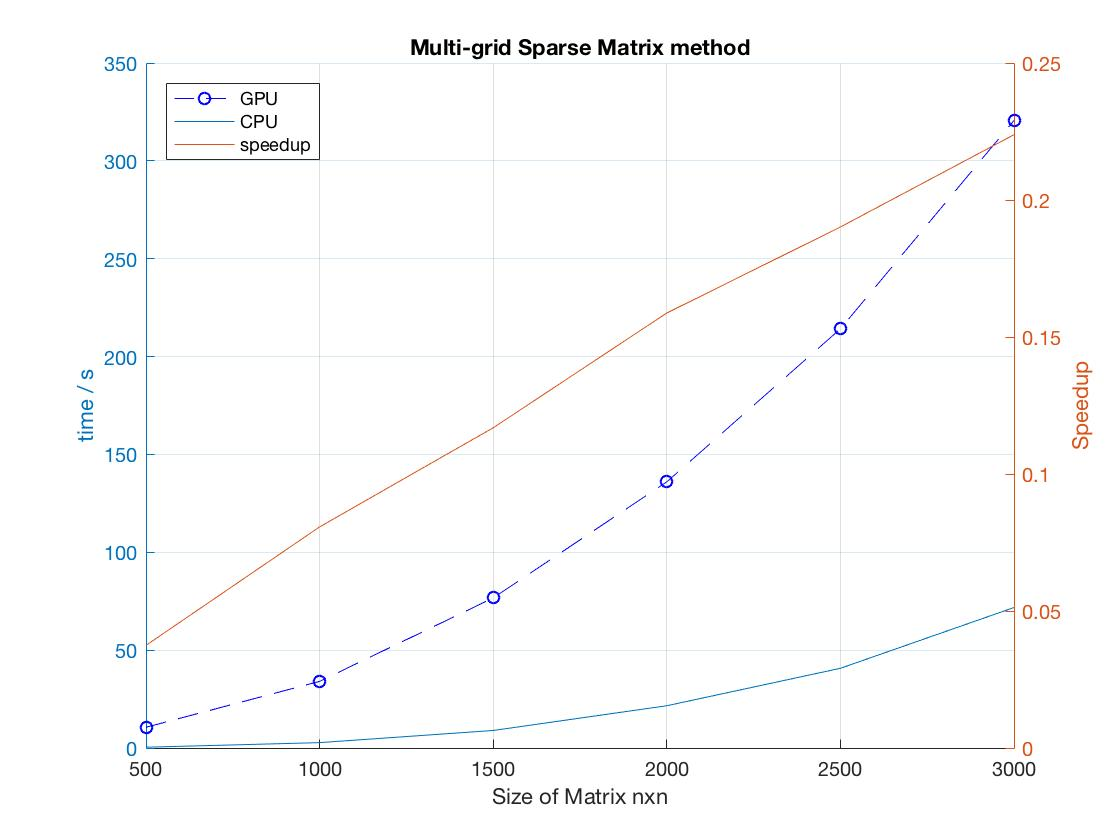
\includegraphics[width = 12cm]{Chapters/multigrid_sparse_matrix.jpg}
	\captionof{figure}{compare OCCA vs CPU performance}
	\label{img:multigridsparse}
\end{center}

%$
%\begin{bmatrix}
%	recursion & size & gputime & cputime & speedup\\
%	8&500&1.97835&0.424889&0.214769\\
%	9&1000&2.30963&2.80448&1.21425\\
%	10&1500&2.7869& 8.92915&3.20398\\
%	10&2000&2.74789&22.0198&8.01333\\
%	11&2500&3.09132&41.114&13.2998\\
%	11&3000&3.2176&68.7087&21.3541\\
%\end{bmatrix}
%$
%
%







%We can see in this graph if matrix size is smaller than 800 than CPU is better than OCCA. And according to size of matrix, the CPU time increase faster also. But OCCA is increase very slightly. In my opinion, OCCA is much better if we have matrix size is bigger than OCCA will be much faster than CPU. 

We can see in this graph \ref{img:multigridsparse} CPU is always faster than OCCA. OCCA, We are call to kernel for each function and copy data also take too much time. We can not implement all the function in kernel, because we do not have any atomic operation in OCCA. We have to return to CPU and call again to kernel. That took too much time. And result, We can see CPU is better than OCCA, but if we consider dense matrix OCCA is better.




\subsection{Numerical analysis of results}
\begin{center}
	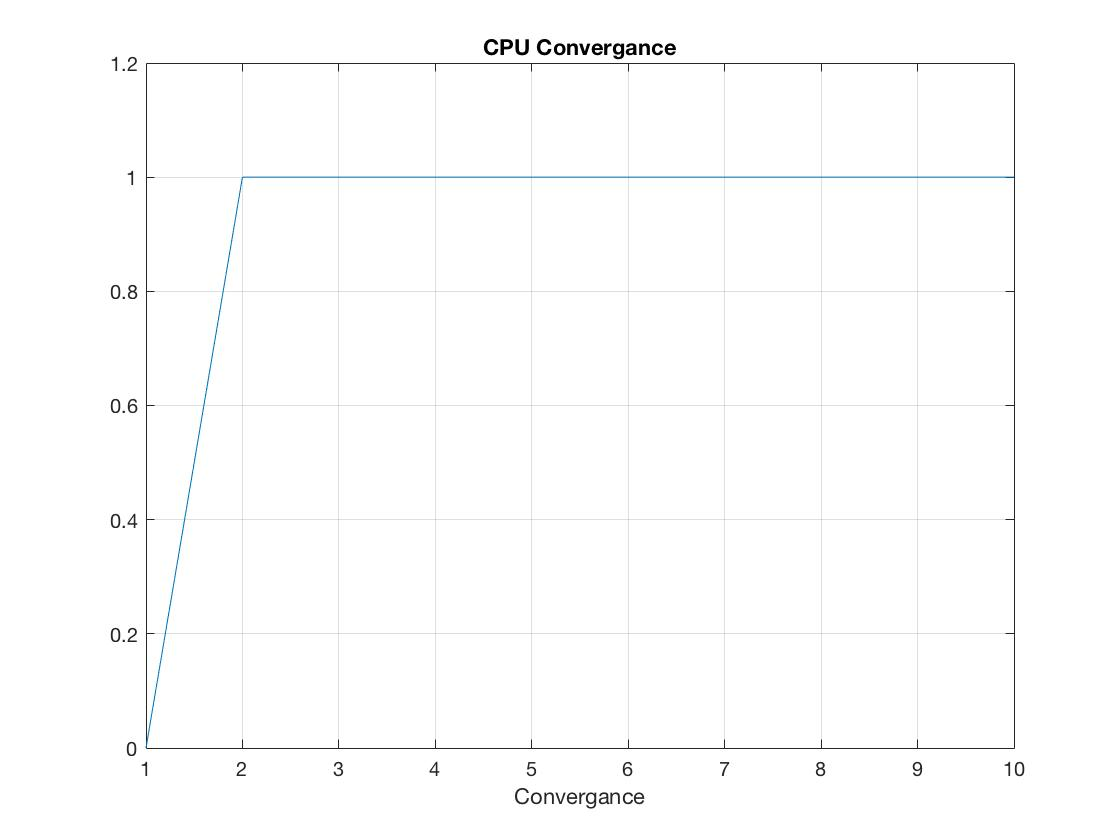
\includegraphics[width = 12cm]{Chapters/cpu_convergence}
	\captionof{figure}{Convergence rate}
	\label{img:convergenceSparse}
\end{center}

This convergence rate \ref{img:convergenceSparse}, which refer to SPD sparse matrix 2000 by 2000 and sparsity ratio is 0.05. We have used 32 bit plotting point. In one Multigrid step, it converge to solution. 













  % Experiment 2

\setcounter{secnumdepth}{-1}
    \chapter{Conclusion}

This thesis, we develop some algorithms with OCCA and C++ by comparing the performances. The time performance of the implementations shows that OCCA with GPU is normally faster than C++ and CPU.  In all cases, the timing results recommend the usage of OCCA instead of the CPU to get  a better performance when the input size of the matrices is large. In our case, We got better performance in all algorithms. But with sparse matrices the performance are not always good. OCCA with GPU is slower than C++ and CPU; because at the moment it not support atomic operation, and other advanced parallel programming features. In some methods, due to OCCA limitation, we can not do parallel computation and we have to return to CPU and call back to kernel that is time consuming.\\
OCCA is easy to use and understand. OCCA uses a syntax similar to C. It has similar for loops (with additional field) and conditional statements. It is good solution, If somebody want to develop parallel applications for different architectures like openCL and CUDA (it works with same code for both architectures). We do not need to write separate code for OpenCL and Cuda. We have shared or exclusive memory operations in OCCA.

The problem of OCCA is that at the moment, the main structure of the project is not completely defined. The biggest problem is the lack of documentation. It has just 2 or 3 slide of documentation and 7 or 8, very short examples. So It is hard to understand, how to implement an optimal kernel.\\
For example in this project, I need atomic operations. But at the moment are not yet supported by OCCA. And the syntax of the kernel is not yet completely defined. For example during the development of this project, the OCCA developers has decided to change a little the syntax of the kernel. And I have spent some time  to  adapt all the methods.

Currently, OCCA developers are working on loop-carried dependency analysis for kernel generation + testing and support offset in kernel calls. They are also developing tiling loop labels for example tile(x,y) and possibly loop-collapsing. And working also on atomic operations. \\

I think OCCA is good solution for parallel programming with GPU. Because an application can works on all different devices like Nvidia, Intel and Radeon GPUs. So the developers are not constrained to a specific family of products. But at the moment, as described, the big problem of OCCA is that is a work progress. So, It is very interesting language, but now, it is not recommendable for long term or big projects.    % Experiment 1

%\chapter{Gaussian elimination}

\section{Introduction}
Gaussian elimination (also known as row reduction) is an algorithm for solving systems of linear equations. It is usually understood as a sequence of operations performed on the corresponding matrix of coefficients. \\
The fundamental idea is to add multiples of one equation to the others in order to eliminate a variable and to continue this process until only one variable is left. Once this final variable is determined, its value is substituted back into the other equations in order to evaluate the remaining unknowns. This method, characterized by step$-$by$-$step  elimination of the variables, is called Gaussian elimination.\\
$\begin{bmatrix}
1&3& \\
2&1&				
\end{bmatrix}$
$\begin{bmatrix}
x \\
y				
\end{bmatrix}$
=
$\begin{bmatrix}
3 \\
5				
\end{bmatrix}$\\

$\begin{matrix}
1x+3y = 3 \\
2x+1y = 5				
\end{matrix}$\\

Multiply row 1 by 2 and subtract from row 2 \\
$\begin{matrix}
1x+3y = 3 \\
5y = 1				
\end{matrix}$\\
$\begin{matrix}
x = 12/5 \\
y = 1/5				
\end{matrix}$
\section{C++ implementation}
The C++ implementation as below:
\begin{lstlisting}[language=C, caption=Gauss elimination in C++]
	void Gauss_elmination_cpu(float a[], float d[], int n) {
	int i, j, k, temp;
	//********* Forward elimination process**************//
	for (int i = 0; i < n - 1; i++) {
		for (int k = i + 1; k < n; k++) {
			float c = a[k * (n + 1) + i] / a[i * (n + 1) + i];
			for (int j = i; j <= n; j++) {
				a[k * (n + 1) + j] = a[k * (n + 1) + j] - (c * a[i * (n + 1) + j]);
			}
		}
	}
    //***************** Backward Substitution method****************//
	for (i = n - 1; i >= 0; i--){
		d[i] = a[i * (n + 1) + n];
		for (int j = i + 1; j < n; j++) {
			if (j != i) {
				d[i] = d[i] - a[i * (n + 1) + j] * d[j];
			}
		}
		d[i] = d[i] / a[i * (n + 1) + i];
	}
}
\end{lstlisting}
\textbf{Forward elimination:} reduction to row echelon form. Using it one can tell whether there are no solutions, or unique solution, or infinitely many solutions.\\
\textbf{Back substitution:} further reduction to reduced row echelon form.\\
In this code, We have i is the row number of matrix and k is walk through all the row which are below the $i^{th}$  row. We have variable c which store the difference of $i^{th}$ row, $i^{th}$ column and $k^{th}$ row, $i^{th}$  column. And j walk through the element of $i^{th}$ and $k^{th}$ row. After finishing this method, We have upper triangular matrix.\\
Which we can solve by backward substitution method. We walk from down to up. We got the value and we use it for solve next value.

\section{OCCA implementation}
Kernel implementation of Guass Elimination is below.
\begin{lstlisting}[language=C, caption=Gauss elimination in OCCA]
    //********* Forward elimination process**************//
    for (int k =i+1; k<n; k++; @tile(16, @outer, @inner)) {
        float c = a[k*(n+1)+i]/a[i*(n+1)+i];
        for (int j=0; j<= n; j++) {
            a[k*(n+1)+j]=a[k*(n+1)+j]-(c*a[i*(n+1)+j]);
        }
    }
}
//***************** Backward Substitution method****************//
  for (int k =0; k < 1; k++; @tile(16, @outer, @inner)) {
        d[i] = a[i*(n+1)+n];
    	for (int j =0; j <n; j++) {
            if (j > i) {
                d[i] = d[i] - (a[i*(n+1)+j] * d[j]);
            }
        }
    	d[i] = d[i]/a[i*(n+1)+i];
    }
}
\end{lstlisting}

In OCCA, We implement the forward substitution and backward substitution method separately. Currently, working dimensions must constant across on all the inner-loops defined in outer loop (@tile(16, @outer, @inner)). In this example k will work in working dimensions. In this case our working dimensions is 16. But the implementation idea is same as CPU implementation.

\section{OCCA vs CPU}
\begin{center}
	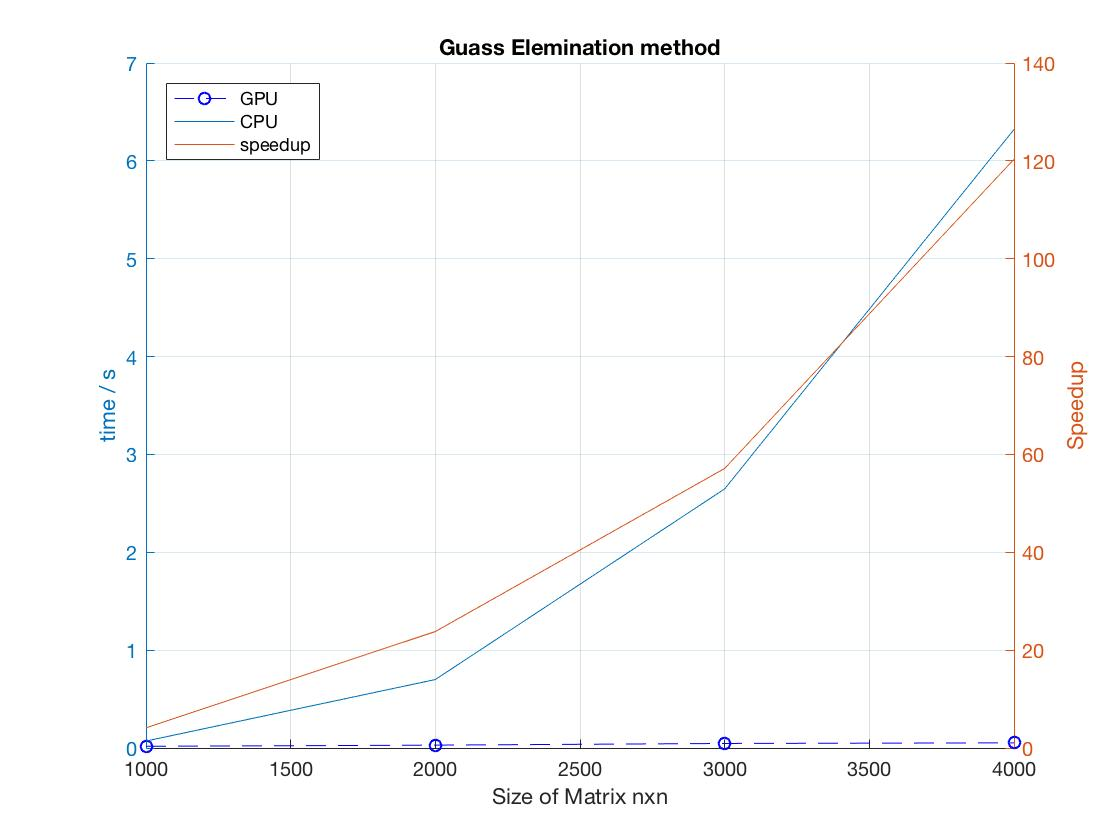
\includegraphics[width = 12cm]{Chapters/guass_elimination.jpg}
	\captionof{figure}{compare OCCA vs CPU performance }
\end{center}

As we can see CPU will more expensive than OCCA. We measure the length of matrix from 500X500 to 4000X4000. And GPU always take time near 0.xxx and CPU takes more time according to length of matrix. According to this conclusion, We can say that OCCA is better than CPU. 


\chapter{Jacobi method}
\section{Introduction}
Jacobi method is an iterative solver used for approximating the solution of diagonally dominant system of linear equations. 
The Jacobi method is easily derived by examining each of the n equations in the linear system Ax = b in isolation. If in the $i^{th}$ equation \\
\begin{equation}
	\sum^n_{j=1}a_{i,j}x_j = b_i
\end{equation}
We solve for the value of $x_i$ while assuming the other entries of x remain fixed, We obtain\\
\begin{equation}
	x_i = (b_i - \sum_{j\neq i}a_{i,j}x_j)/a_{i,i}
\end{equation}
This suggests an iterative method defined by \\
\begin{equation}
	x_i^{(k)} = (b_i - \sum_{j\neq i}a_{i,j}x_j^{(k-1})/a_{i,i}
\end{equation}

Which is the Jacobi method.

\section{C++ implementation}
The C++ implementation as below:
\begin{lstlisting}[language=C, caption=Jacobi method in C++]
	for (int k = 0; k < num_iter; k++) {
		for (int i = 0; i < n; i++ ) {
			float sum = 0;
			for (int j = 0; j < n; j++ ) {
				if ( j != i ) {
					sum += (a[i * (n + 1)+ j] * x[j]);
				}
			}
            x_new[i] = ((a[i * (n + 1) + n]) - sum ) / a[i + i * (n + 1)];
        }
		for (int i = 0; i < n; i++) {
			x[i] = x_new[i];
        }
	}
\end{lstlisting}
This is Jacobi method, Where first loop is count the number of iteration and another loop i,j are start from 0 to n which is the size of the matrix nXn. x is the initial guess vector and x\_new is result vector. And in the last loop, We copy the x\_new to x. It run again and again till k is not equal or bigger than number of iteration.
\section{OCCA implementation}
The OCCA implementation as below:
\begin{lstlisting}[language=C, caption=Jacobi method in OCCA]
	for (int i = 0; i < n; i++; @tile(16, @outer, @inner) ) {
		x_new[i] = a[i * (n + 1) + n];
		float sum =0;
		for (int j = 0; j < n; j++ ) {
			if ( j != i ) {
				sum += a[i + j * (n + 1)] * x[j];
            }
        }
         x_new[i] = ((a[i * (n + 1) + n]) - sum ) / a[i + i * (n + 1)];
        }
        for (int i = 0; i < n; i++; @tile(16, @outer, @inner){
    		x[i] = x_new[i];
    }
\end{lstlisting}
This is OCCA implementation of Jacobi method. It is same as CPU implementation but here we are using the fourth value for for loop. It is @tile(16, @outer, @inner), the tile tag, tiling for-loops as one and two dimensional sets of inner/outer loops. The tile(16) assign the working dimension. In this example it assign the working dimension is 16. 
\section{OCCA vs CPU}
\begin{center}
	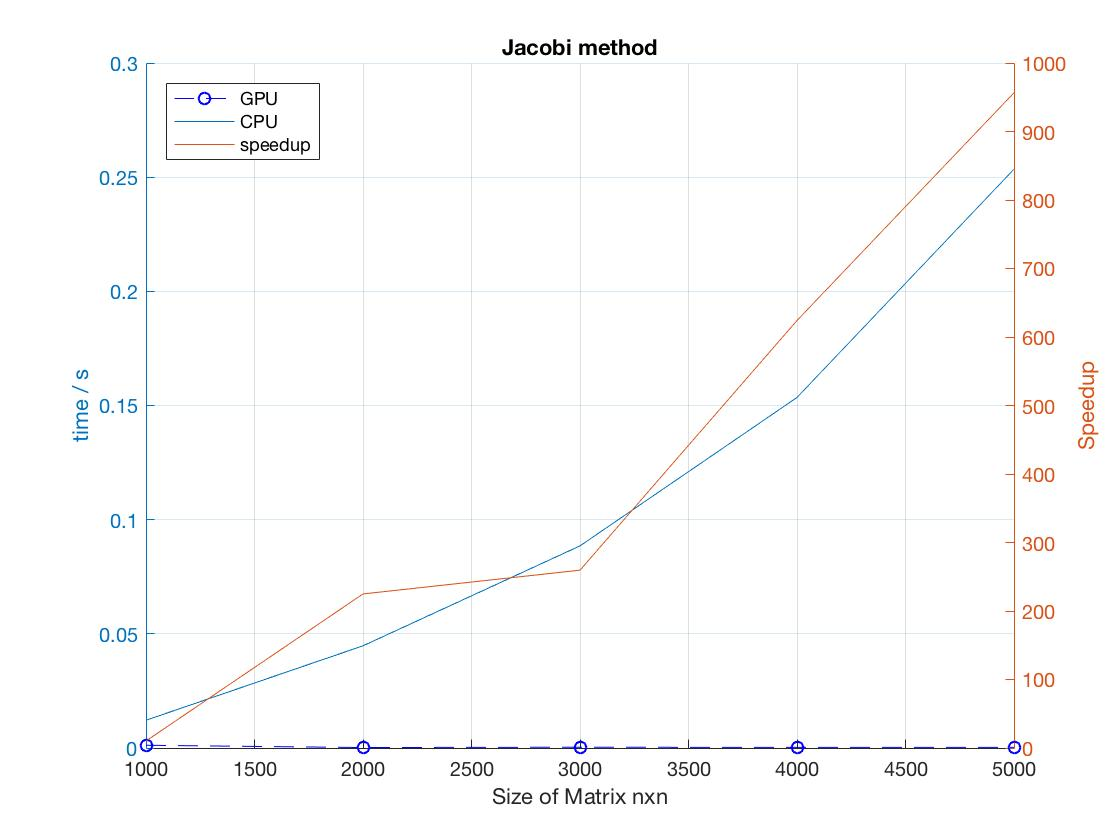
\includegraphics[width = 12cm]{Chapters/jacobi_method.jpg}
	\captionof{figure}{compare OCCA vs CPU performance }
\end{center}

For Jacobi method, OCCA is better than CPU. We can compare according to our results. We compare the matrix size from 1000X1000 to 5000X5000. In this size matrix, OCCA finish the program in 0.xxx time and CPU take time more than 0.2xx and it increase strictly according to size of the matrix.  % Experiment 2

%%\setcounter{secnumdepth}{-1}
    \chapter{Multigrid Method}
    \section{Introduction}
    Multigrid (MG) methods in numerical analysis are algorithms for solving differential equations using a hierarchy of discretizations. They are an example of a class of techniques called multiresolution methods, very useful in problems exhibiting multiple scales of behavior.\\
     The main idea of multigrid is to accelerate the convergence of a basic iterative method (known as relaxation, which generally reduces short-wavelength error) by a global correction of the fine grid solution approximation from time to time, accomplished by solving a coarse problem. From \ref{txt:multigrid}
     
%     \subsubsection{Solution Methods} 
%To solve the systems of linear equations we are using this methods:\\
%• Direct\\
%– Gaussian elimination \\
%• Iterative\\
%– Jacobi\\

\section{Multigrid pseudo-code}

The main structure of a MultiGrid algorithm should be describe by following sequence of operations \ref{eq:main}

\begin{align}
	v^h = MultiGrid(A^h, v^h,f^h,\alpha_1, \alpha_2)
	\label{eq:main} 
\end{align}
\begin{equation}
	Relex\quad \alpha_1 \quad times\quad on\quad A^h u^h = f^h \quad on \quad  \Omega^h \quad with \quad arbitrary \quad initial \quad guess \quad v^h
	\label{eq:relax}
\end{equation}
\begin{equation}
\label{eq:computeB}
	compute \quad residual \quad on \quad  fine \quad  grid \quad r^h = f^h - A^hv^h
\end{equation}
\begin{equation}
\label{eq:computeB2h}
	reduce \quad residual \quad on \quad  coarse \quad  grid \quad r^{2h} = I^{2h}_h r^h
\end{equation}
\begin{equation}
	reduce \quad matrix \quad on \quad  coarse \quad  grid \quad A^{2h} = I^{h}_{2h} A^h I_{h}^{2h}
\end{equation}
\begin{equation}
\label{eq:recursivecall}
	Recursive\quad call\quad to\quad MultiGrid \  to \  solve \quad A^{2h}e^{2h} = r^{2h} \quad on \quad \Omega^{2h}
\end{equation}
\begin{equation}
\label{eq:addx}
	correct \quad fine \quad grid \quad solution \quad v^h = v^h + I_{2h}^he^{2h}
\end{equation}
\begin{equation}
	Relex\quad \alpha_2 \quad times\quad on\quad A^h u^h = f^h \quad on \quad  \Omega^h \quad with \quad v^h
\end{equation}

In this procedure, we relax  $\alpha_1$ times the system of equation $A^h u^h = f^h$ with the given initial guess $v^h$. In this project we use the Jacobi method. We  compute the residuals $r^h$ with the new $v^h$. After that, we  use the reduction operator on $r^h$. We  reduce the matrix $A^h$ by applying the reduction and interpolation operators. Which return $A^{2h}$. Now, We use the recusrion with our new system $A^{2h}e^{2h} = r^{2h}$ to solve system on coarse grid $\Omega^{2h}$. And after that we correct the solution on fine grid $v^h$ by using the correction $e^{2h}$. And finally, we relax with $\alpha_2$ times our $A^h u^h = f^h$ with the initial guess $v^h$.
\section{Multigrid mehtod Dense matrix}

\subsection{Introduction}

In the multi-grid method, We use the Gauss elimination method as exact solver, Jacobi method for relaxation. Some specific functions for matrix interpolation, matrix reduction, vector interpolation. The main idea is \\
\begin{lstlisting}[language=C, caption=multigrid method idea]
	multi-grid method(a, b, x, recursion)
		if (recursion == 0)
			gauss-elimination method(a, b, x)
			return 
		jacobi method(a, b, x, 10)
		
		\\reduction of vector b
		b2h = Reduction (b - a*x)
		
		\\ initialize 
		x2h = 0
		
		\\ compute a2h, R = reduction matrix, I = interpolation matrix
		a2h = R *  a * I
		
		multi-grid method(a2h, b2h, x2h, recursion-1)
		
		xh = interpolation x2h
		
		x = x + xh
		
		jacobi method(a, b, x, 10)
		
\end{lstlisting}
 
With the reduction, We decrease the size of the vector. For example if we have a vector of size n, after reduction we obtain a new vector of size n/2. We call the multi-grid method again with the reduced  $A$, $b$ and $x$. And we repeat this process until the recursion counter is equal to 0; and when it is 0, It calls the Gauss elimination method to solve the given system by stopping the recursive calls.
 

\subsection{C++ implementation}

The C++ implementation as below:\\
\begin{lstlisting}[language=C, caption=Multigrid method in C++]
	if (recursion == 0) {

        Gauss_elmination_cpu(a, b, x, row);
        return ;
    }
    float *x_new2 = new float[row];

    init_zero(x_new2, row);
    jacobi_method_cpu(a, x, b, x_new2, row, alpha);

    float *b2h = new float[row / 2];
    float *res1 = new float[row];
    float *x_new2h = new float[row];
    float *a2h = new float[(row / 2) * (row / 2)];

    init_zero(b2h, row / 2);
    init_zero(res1, row);
    init_zero(x_new2h, row);
    init_zero(a2h, (row / 2) * (row / 2));

    matrix_x_vector(row, row, x, a, x_new2h);

    add_sub_vector(b, x_new2h, res1, row,  -1);

    reduction_vector(res1, (row / 2), b2h);

    init_zero(x_new2h, row);

    interpolation_reduction_matrix(a, row, a2h);

    if (row / 2 <= 0) {
        cout << "error" << endl;
        return;
    }
    multigrid_method(a2h, x_new2h, b2h, recursion - 1, row / 2, alpha);

    float * res_int = new float[(row * 2) + 1];
    init_zero(res_int, (row * 2) + 1);

    reduction_interpolation_vector(x_new2h, row, res_int);
    add_sub_vector(x, res_int, x, row,  1);

    jacobi_method_cpu(a, x, b, x_new2, row, alpha);
\end{lstlisting}

In CPU, It is the same implementation as I describe above. Firstly, We check if the recursion is
0 or not. If yes, we call the Gauss elimination method and stop the recursion. If not,
We call to Jacobi method alpha times. We calculate the $b_h^{2h}$,$x_h^{2h}$  and $a_h^{2h}$. Size of $x_h^{2h}$ is half of size $x_{2h}^h$. And we call multigrid method recusively with the $b_h^{2h}$,$x_h^{2h}$  and $a_h^{2h}$. And subtract 1 from recursion. After recursion call, We convert $x_h^{2h}$ to $x_{2h}^h$ and add in x. In last, We call Jacabi method again alpha time. 


\subsection{OCCA implemintation}
The OCCA implementation as below:\\
\begin{lstlisting}[language=C, caption=multigrid method in OCCA]
	if (recursion == 0) {
        gauss_elmination_call_gpu(row, o_a, o_b, o_x, device);
        return;
    }
    occa::memory o_d, o_b2h, o_x2h, o_a2h, o_res, o_res_result2h;
    // Allocate memory on the device

    o_d  = device.malloc(row * sizeof(float));
    o_b2h  = device.malloc((row / 2) * sizeof(float));
    o_x2h  = device.malloc(row * sizeof(float));
    o_res  = device.malloc(row * sizeof(float));
    o_a2h  = device.malloc((row / 2) * (row / 2) * sizeof(float));
    o_res_result2h  = device.malloc(((row * 2) + 1) * sizeof(float));

    jacobi_method_call_gpu(row, o_a, o_b, o_x, o_d, device, alpha);

    dense_Matrix_Vector_Multiplication_call_gpu(row, o_a, o_x, o_res, device);

    add_sub_call_gpu(row, o_b, o_res, o_res, device, -1);

    relaxation_reduction_vector(row / 2, o_res, o_b2h, device);

    reduction_interpolation_reduction_matrix_call_gpu(row, o_a, o_a2h, device);

    if (row / 2 <= 0) {
        cout << "error" << endl;
        return;
    }

    multigrid_method_gpu(row / 2, o_a2h, o_b2h, o_x2h, device, recursion - 1, alpha);

    relaxation_interpolation_vector_call_gpu(row, o_x2h, o_res_result2h, device);

    add_sub_call_gpu(row, o_x, o_res_result2h, o_x, device, 1);

    jacobi_method_call_gpu(row, o_a, o_b, o_x, o_d, device, alpha);
\end{lstlisting}

It has same idea like CPU implementation, We just make all calculation on OCCA. And we described before Gauss elimination and Jacobi method in OCCA. 

\subsection{OCCA vs CPU}
\begin{center}
	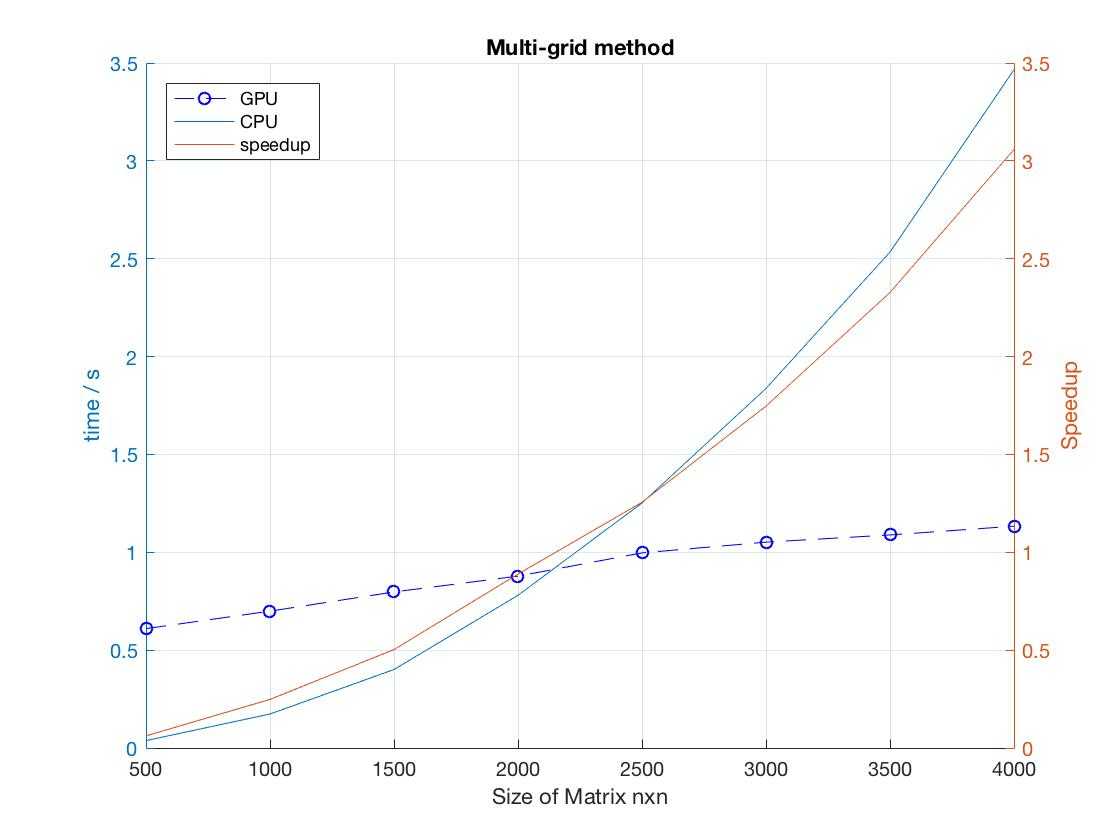
\includegraphics[width = 12cm]{Chapters/multigrid.jpg}
	\captionof{figure}{compare OCCA vs CPU performance}
	\label{img:dmatrix}
\end{center}



In this graph \ref{img:dmatrix} we observe that if the matrix size is small CPU is better than OCCA with GPU. And according to size of matrix, the CPU time increase faster also. But OCCA is increase very slightly. In my opinion, OCCA is much better if the  matrix size is large and OCCA with GPU is faster than CPU. 

\subsection{Numerical analysis of results}
\begin{center}
	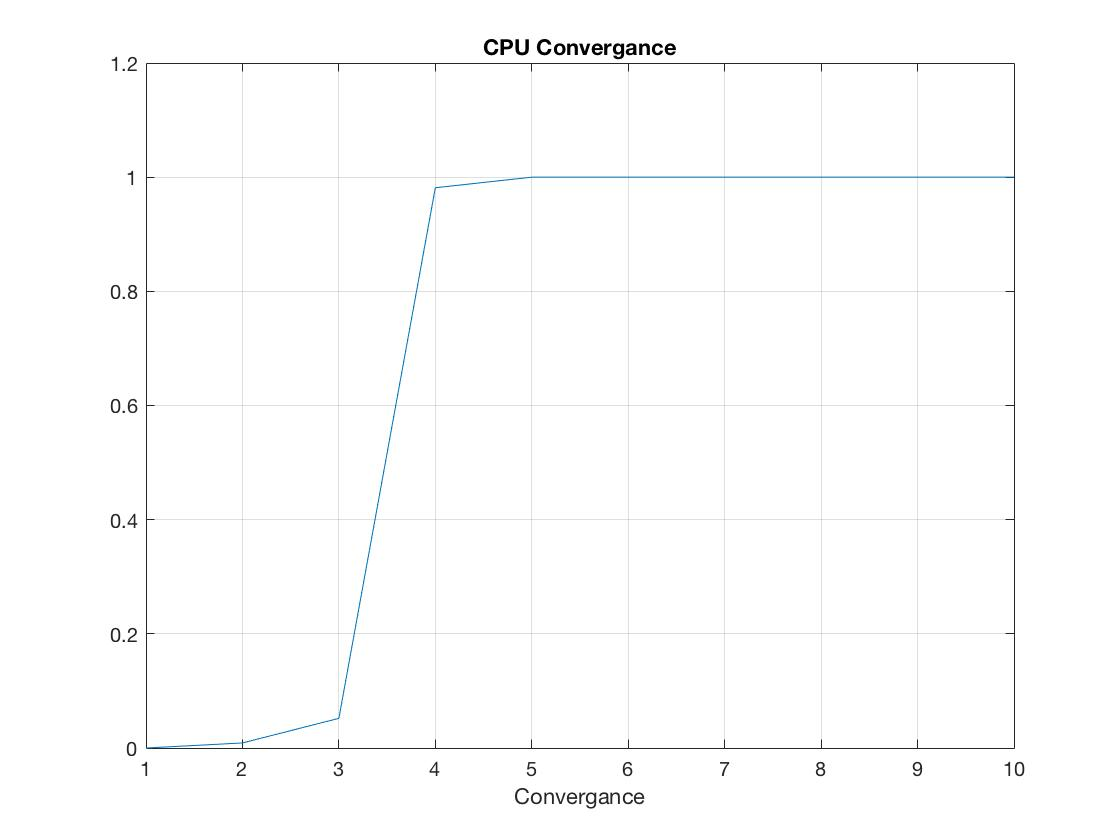
\includegraphics[width = 12cm]{Chapters/cpu_convergence_dense}
	\captionof{figure}{Convergence rate}
	\label{img:convergenceDense}
\end{center}

This convergence rate \ref{img:convergenceDense}, which refer to SPD matrix 2000 by 2000. We have used 32 bit plotting point. In 4s Multigrid step, it converge to solution. 
\section{Multigrid mehtod sparse matrix}
 

\subsection{C++ implementation}

The C++ implementation as below:\\
\begin{lstlisting}[language=C, caption=multigrid method in C++]
	void multigrid_method_sparse_matrix(float a_non_zero[], int a_col_number[], int a_row[], float x[], float b[], int recursion, int row, int alpha, int size_a) {

    if (recursion == 0 || row / 2 < 3 ) {
        int *point = new int[size_a];
        float *aa  = new float [row * row];
        for (int i = 0; i < size_a; i++) {
            point[i] = a_col_number[i] * row + a_row[i];
        }

        vectorToMatrix(row, row, size_a, a_non_zero, aa, point);

        Gauss_elmination_cpu(aa, b, x, row);

        delete [] point;
        delete [] aa;

        return ;
    }


    float *x_new2 = new float[row];
    init_zero(x_new2, row);

    jacobi_method_cpu_sparse_matrix(a_non_zero, a_col_number, a_row, b, x, x_new2, row, alpha, size_a);


    float *b2h = new float[row / 2];
    float *res1 = new float[row];
    float *x_new2h = new float[row];

    init_zero(b2h, row / 2);
    init_zero(res1, row);
    init_zero(x_new2h, row);

    sparse_matrix_x_vector(row, size_a, x, a_row, a_col_number, a_non_zero, x_new2h);
    add_sub_vector(b, x_new2h, res1, row,  -1);
    reduction_vector_sparse(res1, row, b2h);

    init_zero(x_new2h, row);

    int size_non = (size_a + row) * 3;

    float *a2h = new float[size_non];
    int *a2h_row = new int[size_non];
    int *a2h_col = new int[size_non];

    init_zero(a2h, size_non);
    init_zero(a2h_row, size_non);
    init_zero(a2h_col, size_non);


    size_non = interpolation_reduction_matrix_sparse_matrix(a_non_zero, a_col_number, a_row, size_a, row, a2h, a2h_row, a2h_col);

    multigrid_method_sparse_matrix(a2h, a2h_col, a2h_row, x_new2h, b2h, recursion - 1, row / 2, alpha, size_non);

    float * res_int = new float[(row * 2) + 1];

    init_zero(res_int, (row * 2) + 1);

    reduction_interpolation_vector(x_new2h, row, res_int);

    add_sub_vector(x, res_int, x, row,  1);

    init_zero(x_new2, row);

    jacobi_method_cpu_sparse_matrix(a_non_zero, a_col_number, a_row, b, x, x_new2, row, alpha, size_a);


    delete [] x_new2h;
    delete [] b2h;
    delete [] res1;
    delete [] res_int;
    delete [] a2h;
    delete [] a2h_col;
    delete [] a2h_row;
}
\end{lstlisting}

In CPU, It is the same implementation as I describe above. The difference is use of CSR format matrix format rather than use dense matrix with most values 0. Firstly, We check recursion is
0 or not. If yes, we call the Gauss elimination method and stop the recursion. If not,
We call to Jacobi method alpha times. We calculate the $b_h^{2h}$,$x_h^{2h}$  and $a_h^{2h}$. Size of $x_h^{2h}$ is half of size $x_{2h}^h$. And we call multi-grid method recusively with the $b_h^{2h}$,$x_h^{2h}$  and $a_h^{2h}$. And subtract 1 from recursion. After recursion call, We convert $x_h^{2h}$ to $x_{2h}^h$ and add in x. In last, We call jacabi method again alpha time. 


\subsection{OCCA implementation}
The OCCA implementation as below:\\
\begin{lstlisting}[language=C, caption=multigrid method in OCCA]
	void multigrid_method_gpu_sparse_matrix(int row, occa::memory o_a, occa::memory o_a_row, occa::memory o_a_col, occa::memory o_b, occa::memory o_x, occa::device device, int recursion, int alpha, int size_a) {
    if (recursion == 0 || row / 2 <= 3 || size_a < row ) {
        occa::memory o_aa;

        o_aa = device.malloc((row * row) * sizeof(float));

        sparse_vector_to_matrix_gpu_call(row, o_a, o_a_row, o_a_col, device, size_a, o_aa);

        gauss_elmination_call_gpu(row, o_aa, o_b, o_x, device);

        return;
    }

    occa::memory o_b2h, o_x2h, o_a2h, o_a2h_row, o_a2h_col, o_res, o_res2, o_res_result2h, o_row_number ;
    // Allocate memory on the device

    o_b2h  = device.malloc((row / 2) * sizeof(float));
    o_x2h  = device.malloc((row / 2) * sizeof(float));
    o_res  = device.malloc(row * sizeof(float));
    o_res2  = device.malloc(row * sizeof(float));

    int size_non = (size_a + row);
    o_a2h  = device.malloc(size_non * sizeof(float));
    o_a2h_row  = device.malloc(size_non * sizeof(int));
    o_a2h_col  = device.malloc(size_non * sizeof(int));


    jacobi_method_call_gpu_sparse_matrix(row, o_a, o_a_col, o_a_row, o_b, o_x, device,  alpha, size_a);

    sparse_Matrix_Vector_Multiplication_call_gpu(row, size_a, o_a, o_a_row, o_a_col, o_x, o_res, device);

    add_sub_call_gpu(row, o_b, o_res, o_res2, device, -1);

    relaxation_reduction_vector(row / 2, o_res2, o_b2h, device);

    size_non =  reduction_interpolation_reduction_sparse_matrix_call_gpu(row, o_a, o_a_col, o_a_row,  o_a2h, o_a2h_row, o_a2h_col, device, size_a);


    multigrid_method_gpu_sparse_matrix(row / 2, o_a2h, o_a2h_row, o_a2h_col, o_b2h, o_x2h, device, recursion - 1, alpha, size_non);

    o_res_result2h  = device.malloc(((row * 2) + 1) * sizeof(float));

    relaxation_interpolation_vector_call_gpu(row, o_x2h, o_res_result2h, device);

    add_sub_call_gpu(row, o_x, o_res_result2h, o_x, device, 1);

    jacobi_method_call_gpu_sparse_matrix(row, o_a, o_a_col, o_a_row, o_b, o_x, device,  alpha, size_a);
}
\end{lstlisting}

It has same idea like CPU implementation, We just make all calculation on GPU. And we described before Guass elimination and jacobi method in GPU. And, We use the CSR matrix format rather than full matrix size and Gauss elimination method is work only with full matix size. Thats why, We change CSR format matrix to sparse matrix with 0's and than call to Gauss elimination method.

\subsection{OCCA vs CPU}
\begin{center}
	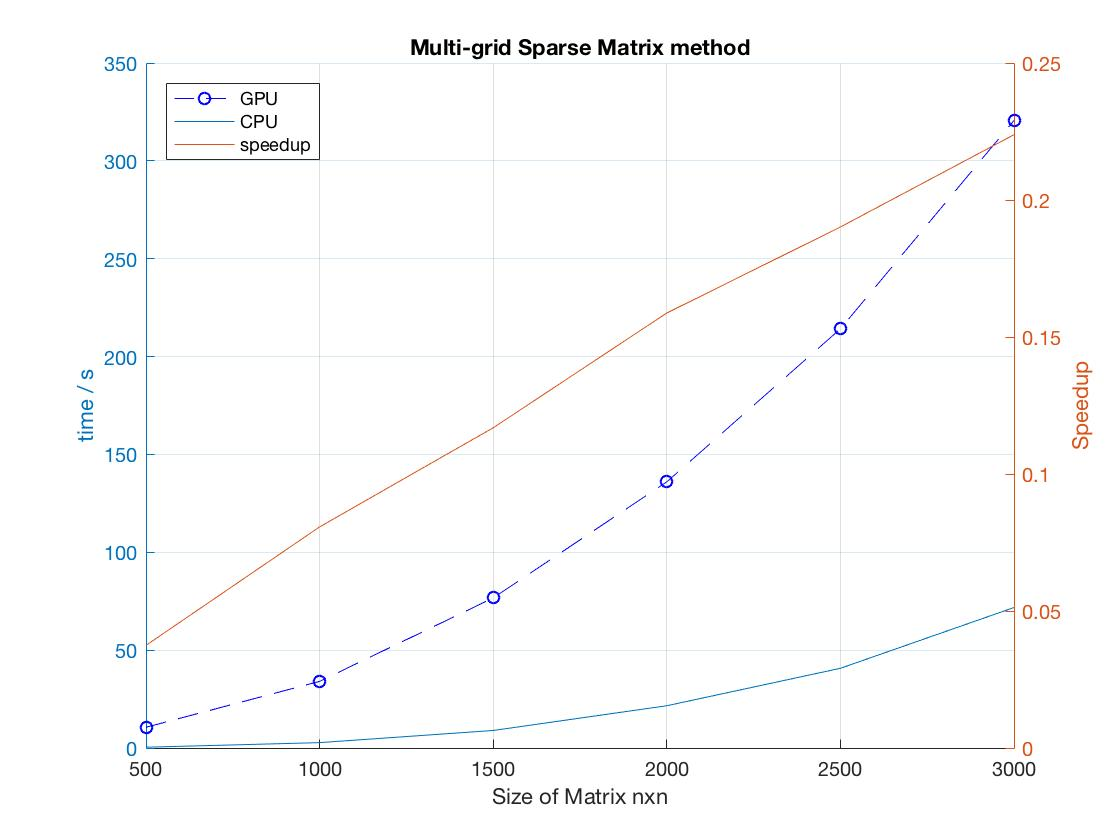
\includegraphics[width = 12cm]{Chapters/multigrid_sparse_matrix.jpg}
	\captionof{figure}{compare OCCA vs CPU performance}
	\label{img:multigridsparse}
\end{center}

%$
%\begin{bmatrix}
%	recursion & size & gputime & cputime & speedup\\
%	8&500&1.97835&0.424889&0.214769\\
%	9&1000&2.30963&2.80448&1.21425\\
%	10&1500&2.7869& 8.92915&3.20398\\
%	10&2000&2.74789&22.0198&8.01333\\
%	11&2500&3.09132&41.114&13.2998\\
%	11&3000&3.2176&68.7087&21.3541\\
%\end{bmatrix}
%$
%
%







%We can see in this graph if matrix size is smaller than 800 than CPU is better than OCCA. And according to size of matrix, the CPU time increase faster also. But OCCA is increase very slightly. In my opinion, OCCA is much better if we have matrix size is bigger than OCCA will be much faster than CPU. 

We can see in this graph \ref{img:multigridsparse} CPU is always faster than OCCA. OCCA, We are call to kernel for each function and copy data also take too much time. We can not implement all the function in kernel, because we do not have any atomic operation in OCCA. We have to return to CPU and call again to kernel. That took too much time. And result, We can see CPU is better than OCCA, but if we consider dense matrix OCCA is better.




\subsection{Numerical analysis of results}
\begin{center}
	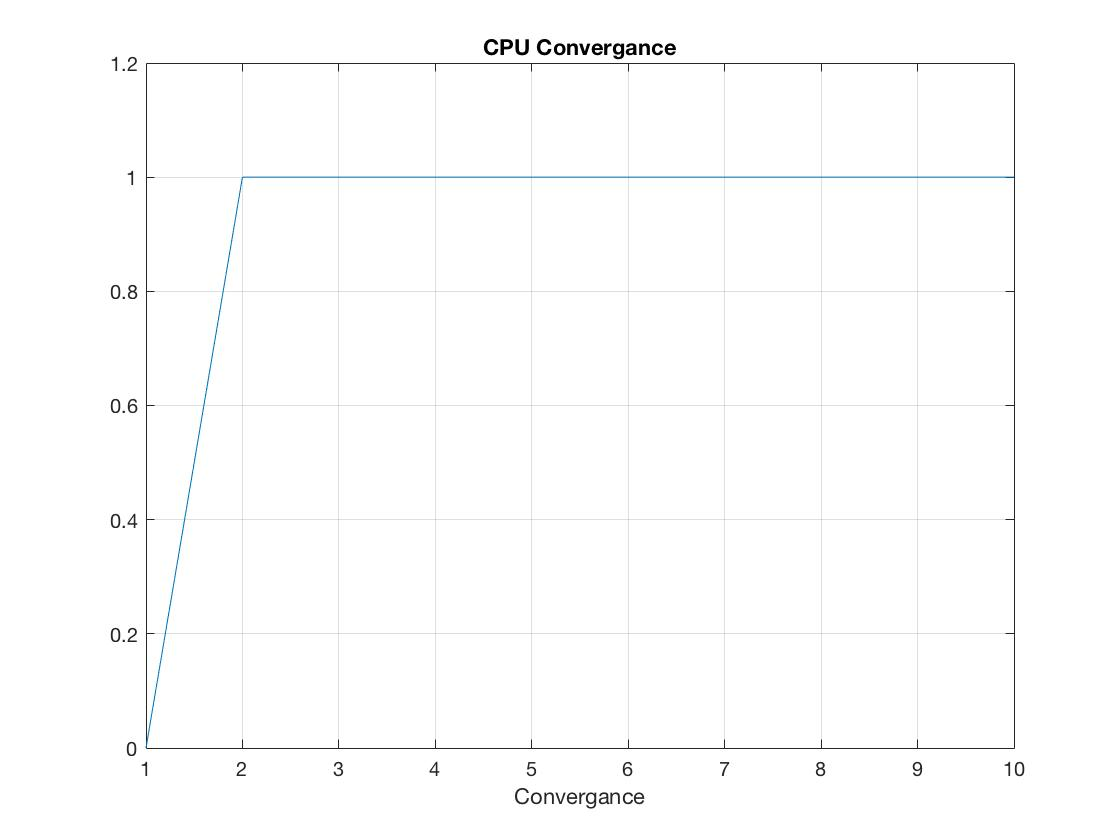
\includegraphics[width = 12cm]{Chapters/cpu_convergence}
	\captionof{figure}{Convergence rate}
	\label{img:convergenceSparse}
\end{center}

This convergence rate \ref{img:convergenceSparse}, which refer to SPD sparse matrix 2000 by 2000 and sparsity ratio is 0.05. We have used 32 bit plotting point. In one Multigrid step, it converge to solution. 













  % Results and Discussion

%\input{Chapters/Chapter7} % Conclusion

%% ----------------------------------------------------------------
% Now begin the Appendices, including them as separate files

\addtocontents{toc}{\vspace{2em}} % Add a gap in the Contents, for aesthetics

\appendix % Cue to tell LaTeX that the following 'chapters' are Appendices

%\chapter{An Appendix}

Lorem ipsum dolor sit amet, consectetur adipiscing elit. Vivamus at pulvinar nisi. Phasellus hendrerit, diam placerat interdum iaculis, mauris justo cursus risus, in viverra purus eros at ligula. Ut metus justo, consequat a tristique posuere, laoreet nec nibh. Etiam et scelerisque mauris. Phasellus vel massa magna. Ut non neque id tortor pharetra bibendum vitae sit amet nisi. Duis nec quam quam, sed euismod justo. Pellentesque eu tellus vitae ante tempus malesuada. Nunc accumsan, quam in congue consequat, lectus lectus dapibus erat, id aliquet urna neque at massa. Nulla facilisi. Morbi ullamcorper eleifend posuere. Donec libero leo, faucibus nec bibendum at, mattis et urna. Proin consectetur, nunc ut imperdiet lobortis, magna neque tincidunt lectus, id iaculis nisi justo id nibh. Pellentesque vel sem in erat vulputate faucibus molestie ut lorem.

Quisque tristique urna in lorem laoreet at laoreet quam congue. Donec dolor turpis, blandit non imperdiet aliquet, blandit et felis. In lorem nisi, pretium sit amet vestibulum sed, tempus et sem. Proin non ante turpis. Nulla imperdiet fringilla convallis. Vivamus vel bibendum nisl. Pellentesque justo lectus, molestie vel luctus sed, lobortis in libero. Nulla facilisi. Aliquam erat volutpat. Suspendisse vitae nunc nunc. Sed aliquet est suscipit sapien rhoncus non adipiscing nibh consequat. Aliquam metus urna, faucibus eu vulputate non, luctus eu justo.

Donec urna leo, vulputate vitae porta eu, vehicula blandit libero. Phasellus eget massa et leo condimentum mollis. Nullam molestie, justo at pellentesque vulputate, sapien velit ornare diam, nec gravida lacus augue non diam. Integer mattis lacus id libero ultrices sit amet mollis neque molestie. Integer ut leo eget mi volutpat congue. Vivamus sodales, turpis id venenatis placerat, tellus purus adipiscing magna, eu aliquam nibh dolor id nibh. Pellentesque habitant morbi tristique senectus et netus et malesuada fames ac turpis egestas. Sed cursus convallis quam nec vehicula. Sed vulputate neque eget odio fringilla ac sodales urna feugiat.

Phasellus nisi quam, volutpat non ullamcorper eget, congue fringilla leo. Cras et erat et nibh placerat commodo id ornare est. Nulla facilisi. Aenean pulvinar scelerisque eros eget interdum. Nunc pulvinar magna ut felis varius in hendrerit dolor accumsan. Nunc pellentesque magna quis magna bibendum non laoreet erat tincidunt. Nulla facilisi.

Duis eget massa sem, gravida interdum ipsum. Nulla nunc nisl, hendrerit sit amet commodo vel, varius id tellus. Lorem ipsum dolor sit amet, consectetur adipiscing elit. Nunc ac dolor est. Suspendisse ultrices tincidunt metus eget accumsan. Nullam facilisis, justo vitae convallis sollicitudin, eros augue malesuada metus, nec sagittis diam nibh ut sapien. Duis blandit lectus vitae lorem aliquam nec euismod nisi volutpat. Vestibulum ornare dictum tortor, at faucibus justo tempor non. Nulla facilisi. Cras non massa nunc, eget euismod purus. Nunc metus ipsum, euismod a consectetur vel, hendrerit nec nunc.	% Appendix Title
%dfsd
%\input{Appendices/AppendixB} % Appendix Title

%\input{Appendices/AppendixC} % Appendix Title

\addtocontents{toc}{\vspace{2em}}  % Add a gap in the Contents, for aesthetics
\backmatter

%% ----------------------------------------------------------------


%\bibliographystyle{unsrt}
\bibliography{sample}
\textbf{Bibliography: }
\begin{enumerate}
  \item \href{https://www.overleaf.com/latex/templates/template-for-a-masters-slash-doctoral-thesis/mkzrzktcbzfl#.WxVLAFOFPOQ}{\LaTeX \quad Template}
  \item \label{txt:multigrid} \href{https://www.researchgate.net/publication/220690328\_A\_Multigrid\_Tutorial\_2nd\_Edition}{A Multigrid Tutorial, 2nd Edition}
  \item \label{txt:mainOCCA} \href{https://libocca.org/}{OCCA}
  \item \label{txt:occa} \href{https://scholarship.rice.edu/bitstream/handle/1911/102233/TR15-04.pdf?sequence=1&isAllowed=y}{OKL: A Unified Language for Parallel Architectures}
  \item \href{http://www.speedup.ch/workshops/w43\_2014/pdf/TimWarburton.pdf}{OCCA: An Extensible Portability Layer for Many-Core Programming}
  \item \label{txt:CSR} \href{http://www.netlib.org/linalg/html\_templates/node98.html}{CRS Matrix-Vector Product}
  \item \href{http://netlib.org/linalg/html\_templates/node91.html}{Compressed Row Storage (CRS)}
  \item \label{txt:sparsematrixformat} \href{https://en.wikipedia.org/wiki/Sparse\_matrix}{Sparse matrix}
  \item \href{https://en.wikipedia.org/wiki/Dot_product}{Dot product}
  \item \href{https://en.wikipedia.org/wiki/Density\_matrix}{Density matrix}
  \item \href{https://arxiv.org/pdf/1403.0968.pdf}{OCCA: A unified approach to multi-threading languages}
	  
	

\end{enumerate}

\end{document}  % The End
%% ----------------------------------------------------------------